\chapter{Bayesian Inference}
\label{Ch:Infer}
In this chapter we present Markov-Chain Monte Carlo (MCMC) algorithms to estimate the Bayesian posterior distribution of the parameters in our Thermogravemetric Analysis (TGA) model. We begin by investigating the effectiveness of this method on a simulated, single reaction TGA. We then apply this to a simulated experiment with two parallel reactions, before applying the algorithm to experimental data. At each stage we look for issues that arise with the algorithm and how to refine this for our application in thermogravemetric modelling. The test cases provides a framework with known parameters and conditions. The key advantage of the simulated data is that we know the underlying parameters and the model predicts exactly the behaviour of our system. For the experimental data we also face the potential issue of model misspesification \cite{KEN01,Bry14}\\

For each application we apply the same basic statistical model. Let, $F(\theta_M)$ denote the vector corresponding to the solution of the relevant ODE equation, evaluated at the times, $t$. The symbol, $\theta_M$ denotes
the parameters required for the differential equation. The simulated data, $y$ is generated by, adding Gaussian noise to the simulation. Our liklihood function is, 
\begin{equation}
\textbf{y}~ \sim ~N\left(\textbf{F}\left(\theta_{M}\right),\sigma^2\textbf{I}\right). \label{eqn:liklihood}
\end{equation}
To evaluate this liklihood we are required to solve the ODE equation. We solve the ODE numerically using a simple Runge-Kutta algorithm. The posterior distribution follows the equation,
\begin{equation}
P(\theta|\textbf{y})=\frac{P(\textbf{y}|\theta)P(\theta)}{\int P(\textbf{y}|\theta)P(\theta) d\theta},
\end{equation}
where, $\theta=\left(\theta_M,\sigma\right)$ represents our parameters, $P(\textbf{y}|\theta)$ follows the liklihood function in Equation \ref{eqn:liklihood}, and $P(\theta)$ is the prior for our parameters which generally a uniform distribution. $P(\textbf{y})=\int P(\textbf{y}|\theta)P(\theta) d\theta$ is a normalising constant, sometimes referred to as the model evidence. Since the likelihood \ref{eqn:liklihood} requires the solution to the ODE, $P(\textbf{y})$ is unavailable in closed form. Instead we use MCMC methods to simulate from the posterior $P\left(\theta|\textbf{y}\right)$.\\
\begin{algorithm}[H]
\SetAlgoLined
\KwResult{Write here the result }
 Initialise $\theta$ by sampling from the prior\;
 \While{sample_size $<$ required sample}{
  Sample $\theta ^*~ \sim ~ Q(theta^*|\theta)$ \;
  Set $\alpha = \frac{P(\textbf{y}|\theta^*)Q(\theta_{t-1}|\theta^*)P(\theta^*)}{P(\textbf{y}|\theta)Q(\theta^*|\theta_{t-1})P(\theta_{t-1})}$\;
  Sample $b ~ \sim ~U(0,1)$\;
  \eIf{$\alpha>b$}{
   Set $\theta_t=\theta^*$} {
   Set $\theta_t=\theta_{t-1}$
   }
 }
 \caption{Metropolis Hastings Algorithm}
 \label{Alg:MH}
\end{algorithm}
The MCMC algorithm we use is a Metropolis-Hastings Algorithm outline in Algorithm \ref{Alg:MH}. Our algorithm proposes new parameters, $\theta ^*$, using a Gaussian random walk proposal, centered on the previous parameters. This proposal has the advantage of being symmetric, $Q(\theta |\theta^*)=Q(\theta^*|\theta)$. This reduces the amount of computations that are required when determining the likelihood, $\alpha$ in Algorithm \ref{Alg:MH}.\\ 
We have not yet defined the variance of the Gaussian proposal distribution. When selecting this variance it is important to consider what acceptance rate is acceptable. If the acceptance rate is too large, then the algorithm may not have explored enough of the parameter space. A low acceptance rate increases the number of iterations required to generate our sample. There are numerous ways to consider the optimal acceptance rate. Roberts et al. \cite{Rob97} and Yang et al. \cite{Yang20}  indicates that an acceptance rate of 0.234 can be obtained under some conditions. Achieving a rate similar to this over the course of the algorithm is unlikely. At different stages of the algorithm we want different acceptance rates. In an ideal case, the early stages of the algorithm quickly locates the maximum likelihood point. To achieve this a large variance is considered. Once the algorithm is near this local maximum more precise steps are required to generate a sample from the posterior distribution. We vary the variance to allow greater steps to occur initially and smaller steps to occur later in the algorithm.\\
The initial values proposed in the algorithm are heavily dependant upon the starting point. At this stage, known as the transition phase, the algorithm has yet to converge and is not approximating the posterior distribution. These values are considered the burn in for the algorithm and must be discarded. Our algorithm is set up so that a fixed number of points are proposed. To discard the burn in points we take a fixed sample size from the end of the chains and discard all but the last 1000 values.\\
The algorithm is dependant upon the starting values. In our simulations we create four chains, each with different starting values. Each chain follows the same process outlined in Algorithm \ref{Alg:MH}. This is particularly important when the posterior distribution has multiple modes. This is also a key advantage of using the MCMC approach as traditional optimisation methods can become stuck in the suboptimal modes. %cite

\section{Single Reaction}
\label{Sec:1R}
To develop the MCMC algorithm, we need to define our model and model parameters. We use the model
\begin{align}
\frac{dM}{dt}&=-MOA\exp\left(\frac{-E}{RT}\right), \label{TGA_system_BI} \\
\frac{dT}{dt}&=\alpha, \label{TGA_system2_BI}
\end{align}
derived in section \ref{SEC:TGA}. In this application since the oxygen level does not change, then this constant is absorbed into the pre-exponential factor $A$.\\
Using this model, we consider the parameters $A$ and $E$. We also need a parameter $\sigma$ that represents the noise of our data. We set the true parameters to be $A_{\text{true}}=3.17\times10^6 \text{min}^{-1}$, $E_{\text{true}}=8.616\times 10^4 \text{J}/\text{mol}$, and $\sigma_{\text{true}}=0.05$. Since the parameters $A$ and $E$ can vary significantly on a log scale we explore the parameter space using the parameters, $\tilde{E}=\log_{10}E$ and $\tilde{A}=\log_{10}A$. This is a key transformation allowing the algorithm to explore many orders of magnitude much more easily than if we used the original variables. This can reduce the burn in time and provide greater precision. Our vector of parameters, $\theta$, in Algorithm \ref{Alg:MH} becomes $\theta=\left(\tilde{E},\tilde{A},\sigma\right)$.\\
We require a prior and proposal distribution for our parameters. In the absence of any additional information, the simplest choice is to use an uninformative uniform distribution over the parameters $\tilde{A}$ and $\tilde{E}$. As we are using the parameter space of these variable in our algorithm, this reduces some of the calculations. This choice of prior equates to a log-uniform distribution over the variables $A$ and $E$. As stated in at the beginning of this chapter, we use a Gaussian proposal distribution around the previous estimates, which reduces the number of calculations we require. Specification of these distributions are stated in Appendix \ref{App:Distributions}.\\
Simulating the single reaction using the true parameters and adding some noise we obtain the mass curve in Figure \ref{fig:single_mass}. For the single reaction we limit our discussions to include only the mass of the reactant, rather than a sample mass. Converting to a sample mass is a simple manipulation of the same curve.\\
\begin{figure}[h!]
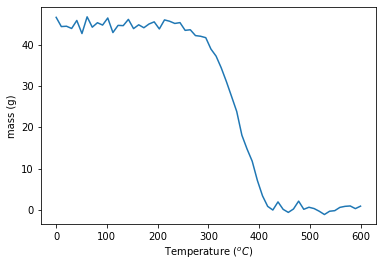
\includegraphics[scale=1]{figures/bayesian/Noisy_tga.png}
\caption{Sample noisy experimental data.}
\label{fig:single_mass}
\end{figure}

The random sample of parameter estimates obtained through the MCMC algorithm are displayed in Figures \ref{HistA} and \ref{HistE}. These histograms are indicative of the posterior distribution. We can use this data to analyse the posterior distribution to obtain point estimates and confidence intervals for the parameters. The ability to apply a functional transformation of our sampled data allows us to utilise these estimates for $\tilde{A}$ and $\tilde{E}$ to determine the critical stockpile lengths required for stockpile ignition. This is a significant advantage of the Bayesian approach. \\ 
\begin{figure}[h!]
\centering
\begin{subfigure}{0.5\textwidth}
\centering
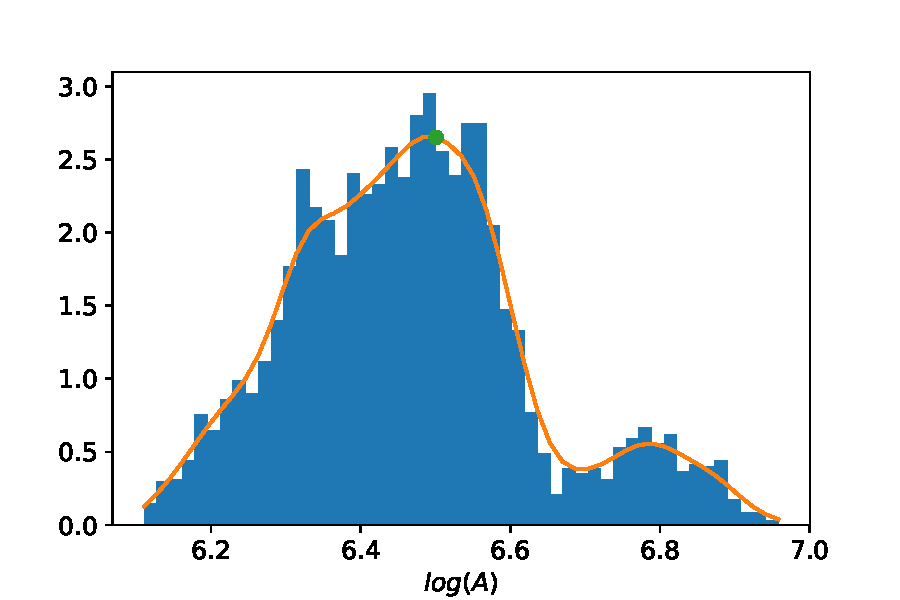
\includegraphics[width=\linewidth]{figures/bayesian/hist_A.pdf}
\caption{Histogram of $\tilde{A}$.}
\label{HistA}
\end{subfigure}%
\begin{subfigure}{0.5\textwidth}
\centering
\includegraphics[width=\linewidth]{figures/bayesian/hist_E.pdf}
\caption{Histogram of $\tilde{E}$.}
\label{HistE}
\end{subfigure}
\newline
\begin{subfigure}{0.5\textwidth}
\centering
\includegraphics[width=\linewidth]{figures/bayesian/hist_sigma.pdf}
\caption{Histogram of $\sigma$.}
\label{Histsigma}
\end{subfigure}%
\begin{subfigure}{0.5\textwidth}
\centering
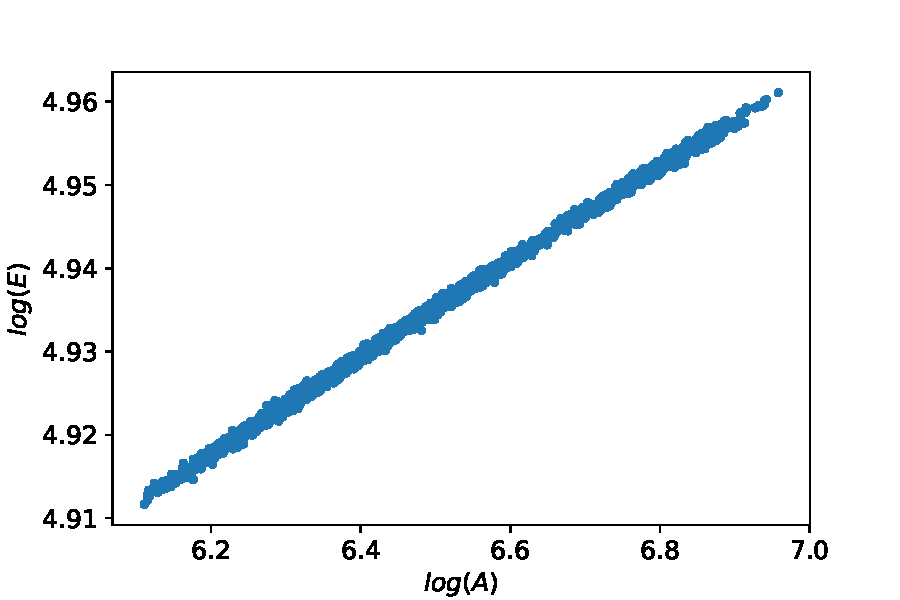
\includegraphics[width=\linewidth]{figures/bayesian/joint_distribution.pdf}
\caption{Joint distribution of $\tilde{A}$ and $\tilde{E}$.}
\label{AvsE}
\end{subfigure}
\caption{Output from the Metropolis-Hastings algorithm with the true values indicated.}
\label{fig:MH1}
\end{figure}

Figure \ref{fig:MH1} displays the sample density that our Metropolis-Hastings Algorithm generates. In each Histogram we capture the true value within the bounds of our sample. We can construct confidence intervals for the true parameters based off our samples. Given we have the true values we can calculate the percentile of each value and these are stated in Table \ref{tab:MH1}. Various summary statistics were calculated and can be found in Appendix \ref{App:1_Summary}.\\ 
\begin{table}[h!]
\centering
\begin{tabular}{|c|c|c|}
\hline 
Parameter & True Value & Percentile \\
\hline
$\tilde{E}$ & 4.94 & 89.7 \\
\hline
$\tilde{A}$ & 6.5 & 89.5 \\
\hline
$\sigma$ & 0.05 & 0\\
\hline
\end{tabular}
\caption{Table of the percentile scores from the Metropolis-Hastings Algorithm.}
\label{tab:MH1}
\end{table}

%Add figure for the histogram of Sigma.
Figure \ref{Histsigma} indicates that the 4 chains have not converged and that no chain has estimated the true noise. This presents a major issue with our algorithm. Figure \ref{fig:trace1} displays the trace plots for the parameters $\tilde{A}$ and $\tilde{E}$. The figure indicates that some chains take significantly longer to converge. This causes issues in determining the appropriate number of samples to accept before terminating the algorithm. This is also a reason why the sigma values are comparatively large. If the sampled points produce a FWC curve that is not sufficiently close to the data, then increasing the noise parameter increases the likelihood. Additional figures for the trace plots of each parameter are included in Appendix \ref{App:1_traces}.
\begin{figure}[h!]
\centering
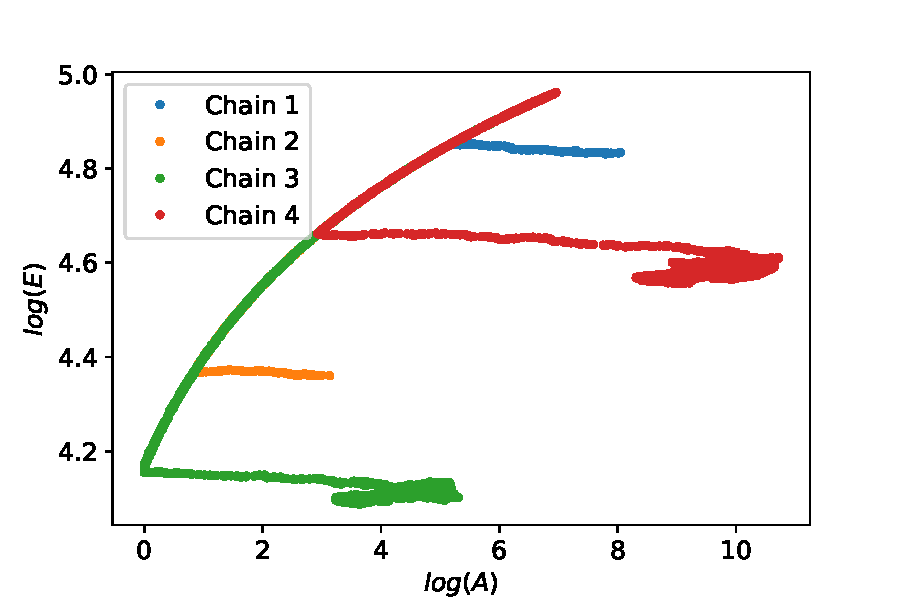
\includegraphics[width=\linewidth]{figures/bayesian/trace_plots.pdf}
\caption{Trace plots of the parameters $\tilde{A}$ and $\tilde{E}$, for each chain.}
\label{fig:trace1}
\end{figure}

Figure \ref{AvsE} plots the joint distribution of the parameters $\tilde{E}$ and $\tilde{A}$. This indicates that the two variables are highly correlated, with correlation coefficient, $0.99$. The fact that the variables are highly correlated causes inefficiencies in the MCMC algorithm.
Given that this curve is so signifant in the acceptance of new data points, it is useful to design an algorithm that samples along this curve. When we propose $\tilde{A}$ and $\tilde{E}$ independently, it is unlikely to remain on this curve.\\
Consider Equation \ref{eqkis},
\begin{equation}
A\exp\left(\frac{-E}{RT_m}\right)=\frac{E}{RT_m^2}\frac{dT}{dt}, \label{eqkis}
\end{equation}
derived in section \ref{SEC:TGA}.
This equation relates the pre-exponential factor ,$A$, and activation energy, $E$, to the temperature at which the reaction rate is maximised, $T_m$. Figure \ref{fig:eqkis_comp} compares the points sampled by our original algorithm with the theoretical true curve with $T_{m,\text{true}}=635$K. We observe that the Markov Chains follow this curve quite closely. Using this information it would be more beneficial to propose new parameters along these curves. The issue remains in how to identify which of these curves do we sample along.\\
\begin{figure}[h!]
\centering
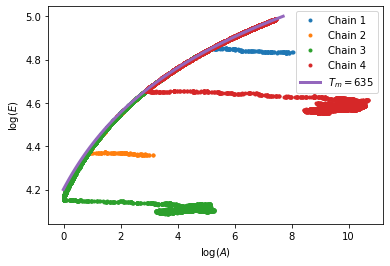
\includegraphics[width=\linewidth]{figures/bayesian/Theoritcal_Tm.png}
\caption{A comparison of the sampled points and the curve in equation \ref{eqkis}.}
\label{fig:eqkis_comp}
\end{figure}

Using Equation \ref{eqkis} alleviates another issue with our sampling method; We do not have good prior information on either the pre-exponential factor nor the activation energy. This equation allows us to replace the parameter $\tilde{A}$ from our sample space with the parameter $T_m$. We propose $T_m$ and $\tilde{E}$ values, and then using Equation \ref{eqkis} we determine the corresponding $\tilde{A}$ value. In the case where we have one reaction, we can often measure $T_m$ directly from the experimental data. For this simulation we do not wish to use this explicit value as we intend to apply this to a scenario with two reactions where we are unable to determine the value explicitly. Even without knowing the exact value, we are able to obtain a useful prior distribution for $T_m$. We use a uniform prior with a limited range.\\
%Include additional figures for the new histograms. Also provide histograms for the original parameters.
\begin{figure}[h!]
\centering
\begin{subfigure}{0.5\textwidth}
\centering
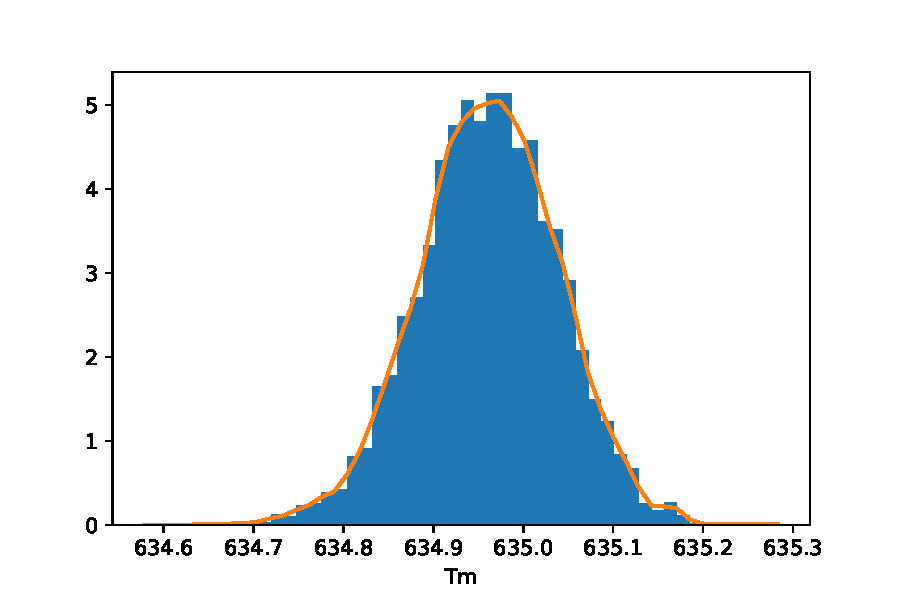
\includegraphics[width=\linewidth]{figures/bayesian/Tm/hist_Tm.pdf}
\caption{Histogram of $T_m$}
\label{HistTm}
\end{subfigure}%
\begin{subfigure}{0.5\textwidth}
\centering
\includegraphics[width=\linewidth]{figures/bayesian/Tm/hist_E.pdf}
\caption{Histogram of $\tilde{E}$}
\label{HistTE}
\end{subfigure}
\newline
\begin{subfigure}{0.5\textwidth}
\centering
\includegraphics[width=\linewidth]{figures/bayesian/Tm/hist_sigma.pdf}
\caption{Histogram of $\sigma$}
\label{HistTsigma}
\end{subfigure}%
\begin{subfigure}{0.5\textwidth}
\centering
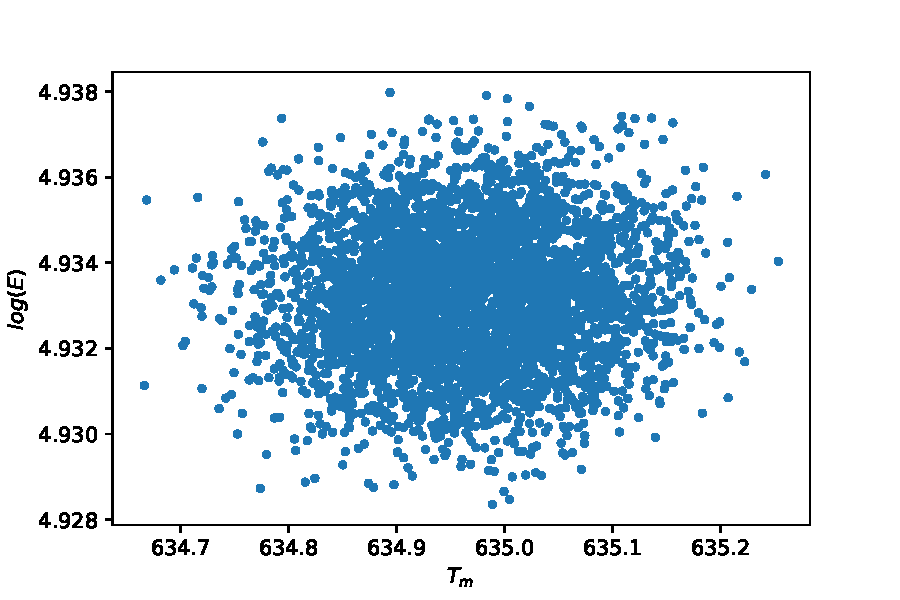
\includegraphics[width=\linewidth]{figures/bayesian/Tm/joint_distribution.pdf}
\caption{Joint distribution of $T_m$ and $\tilde{E}$.}
\label{TvsE}
\end{subfigure}
\caption{Output from the Metropolis-Hastings algorithm using the parameters $(T_m,E)$, with the true values indicated.}
\label{fig:MH2}
\end{figure}

%Look to include traceplots and additional information on
Using the parameter $T_m$, we obtain very similar graphs for $A$ and $E$. The plot for $E$ against $T_m$ is displayed in figure \ref{TvsE}. This figure indicates that there is no significant correlation between the two parameters. This is useful in our algorithm as it improves the acceptance rate with similar step sizes. This is further supported by the trace plot in figure \ref{fig:trace2}.\\
\begin{figure}[h!]
\centering
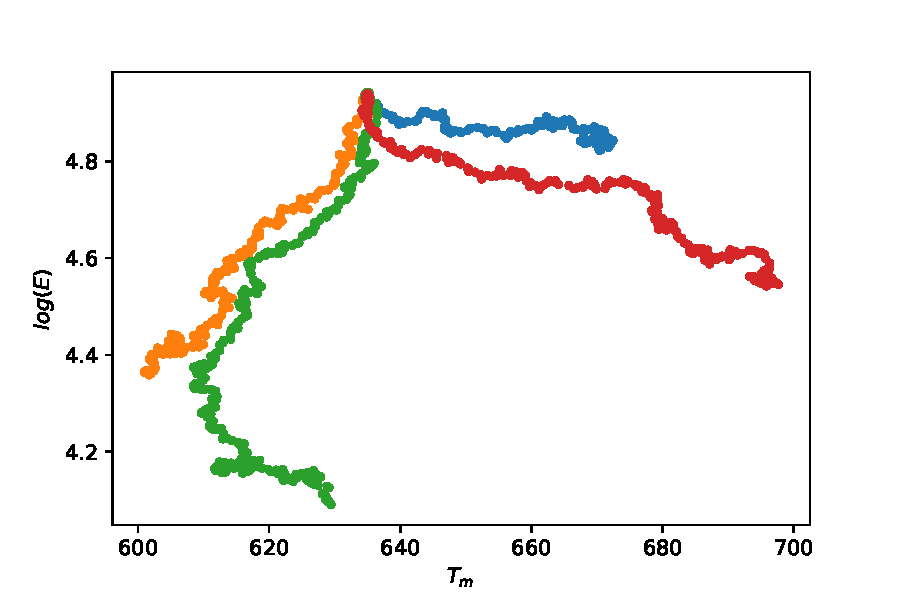
\includegraphics[width=\linewidth]{figures/bayesian/Tm/trace_plots.pdf}
\caption{Trace plots of the parameters $T-m$ and $\tilde{E}$, for each chain.}
\label{fig:trace2}
\end{figure}
One of the key metrics we are interested in is the effect that this variation has on the predicted critical length of the stockpile. This is a major benefit of the MCMC approach as we can conduct a functional transform from our sample to the critical length using the formula,
\begin{equation}
L_{cr}=K \sqrt{\frac{\exp\left(\frac{E}{RT_a^2}\right)}{A}\frac{RT_a^2}{E}},
\label{eq:Lcr}
\end{equation}
where $K$ is some constant that depends upon various constants in our stockpile model. Equation \ref{eq:Lcr} was derived in Section \ref{SEC:Lcr}. We have taken this constant such that the minumum critical length is $1$m.
Figure \ref{fig:HistL} indicates that the critical length of the stockpile can be determined to within some reasonable range. The values in the histogram are indicative of the critical lengths and are dependant on the thermal conductivity and the heat of reaction; these parameters are not included in our TGA analysis. Using Equation \ref{eq:Lcr} and taking logarithms we obtain,
\begin{equation}
\log \left(L_{cr}\right)=\log (K)+\log\left(\frac{RT_a^2}{EA}\right) +\frac{E}{RT_a^2}\log( e).
\end{equation}
This form clearly indicates that the parameter, $K$ shifts the values of $\log L_{cr}$ and does not affect the spread.\\
\begin{figure}
\centering
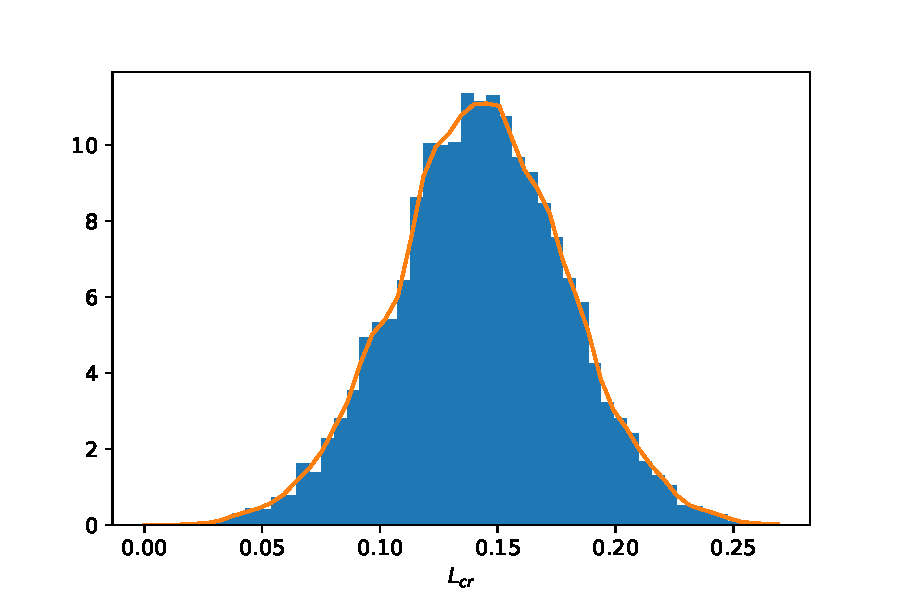
\includegraphics[scale=1]{figures/bayesian/hist_Lcr.pdf}
\caption{Histogram of the sample obtained for $\log_{10}\left(L_{\text{cr}}\right)$ through the MCMC algorithm.}
\label{fig:HistL}
\end{figure}
\subsubsection{Selecting Appropriate Parameters}
This section has shown that utilising a different set of parameters can improve the efficiency of the MCMC algorithm. It is useful to consider why this is the case.\\ 
\begin{figure}[h!]
\centering
\begin{subfigure}{.5\textwidth}
  \centering
  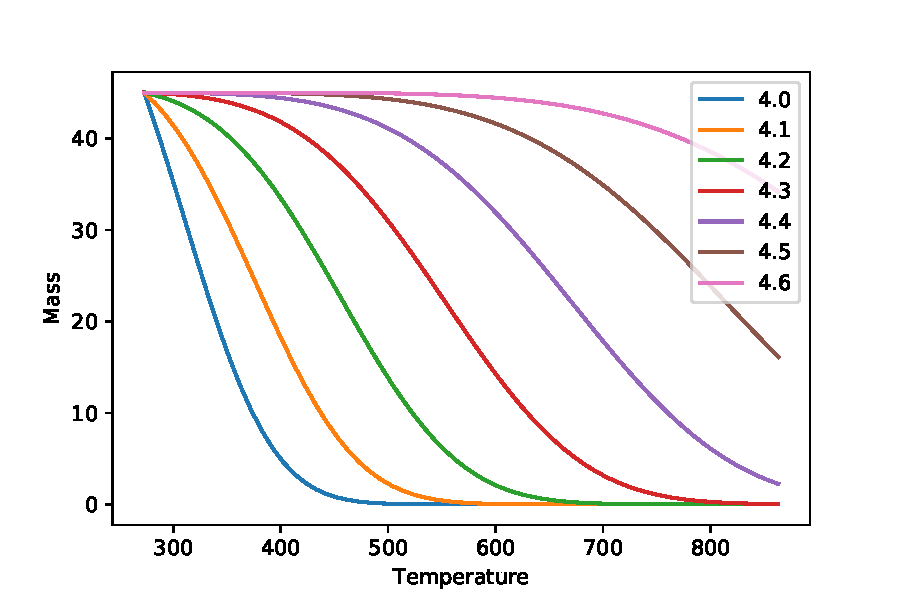
\includegraphics[width=\linewidth]{figures/bayesian/1_reaction/E_A_fwc.pdf}
  \caption{The effect of $\tilde{E}$ with $\tilde{A}=6$.}
  \label{fig:subfwc_E_A}
\end{subfigure}%
\begin{subfigure}{.5\textwidth}
  \centering
  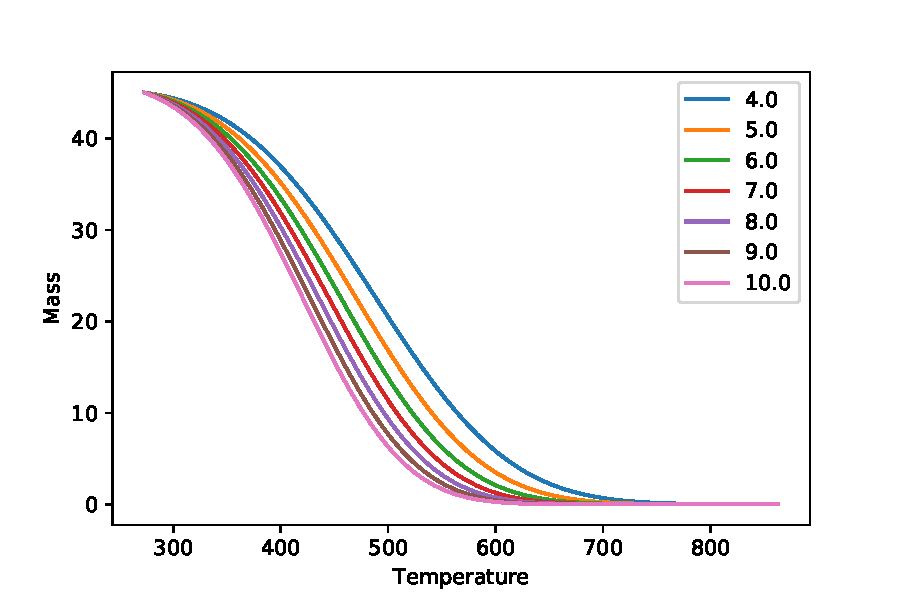
\includegraphics[width=\linewidth]{figures/bayesian/1_reaction/A_fwc.pdf}
  \caption{The effect of $\tilde{A}$ with $\tilde{E}=4.2$.}
  \label{fig:subfwc_A_E}
\end{subfigure}
\newline
\begin{subfigure}{.5\textwidth}
  \centering
  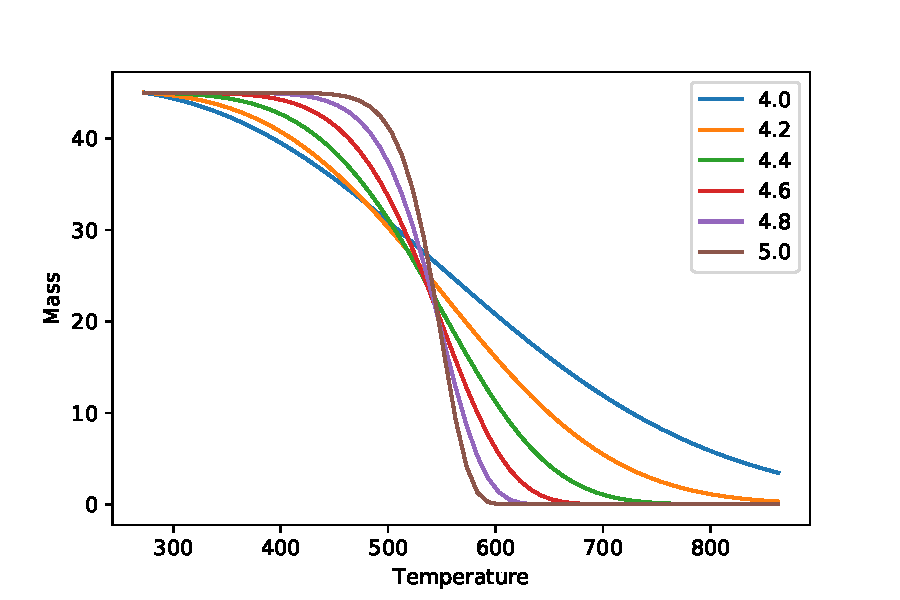
\includegraphics[width=\linewidth]{figures/bayesian/1_reaction/E_fwc.pdf}
  \caption{The effect of $\tilde{E}$ with $T_m=550$.}
  \label{fig:subfwc_E_Tm}
\end{subfigure}%
\begin{subfigure}{.5\textwidth}
  \centering
  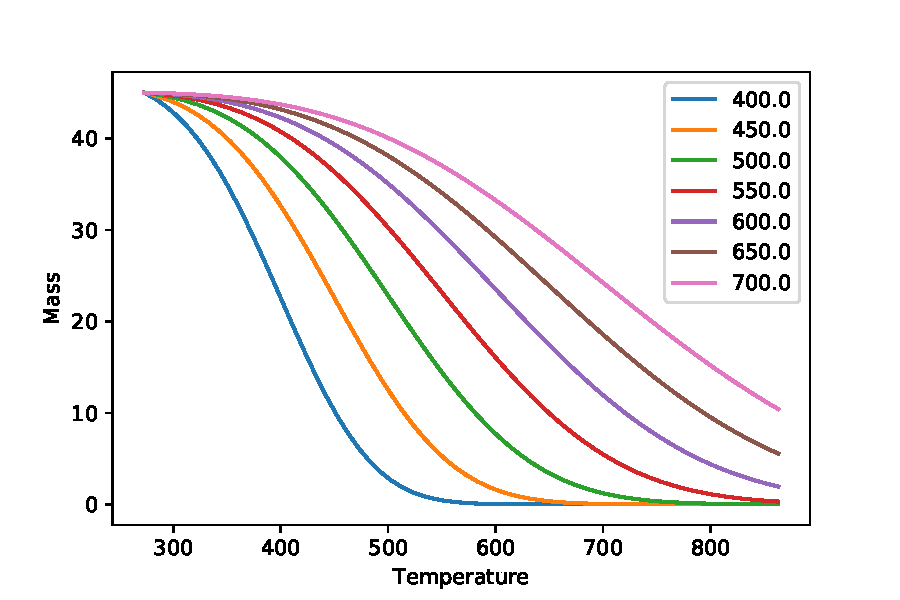
\includegraphics[width=\linewidth]{figures/bayesian/1_reaction/Tm_fwc.pdf}
  \caption{The effect of $T_m$ with $\tilde{E}=4.2$.}
  \label{fig:subfwc_Tm_E}
\end{subfigure}
    \caption{Comparison of the effects of each parameter pairing on the FWC curve.}%
    \label{fig:FWC_para_comp}%s}
\end{figure}%
Figure \ref{fig:FWC_para_comp} demonstrates the effect that altering each parameter has on the FWC curve. We observe in figures \ref{fig:subfwc_E_A} and \ref{fig:subfwc_A_E}, that the $\tilde{E}$ parameter has a large effect on both when the reaction occurs and its duration; small changes in $\tilde{E}$ cause a large shift in the FWC curve. In contrast the affect of changing $\tilde{A}$ appears to be minimal. Dramatically changing the order of magnitude of the parameter has little effect on FWC curve. This is in contrast to the $\left(\tilde{E},T_m\right)$ pairing displayed in figures \ref{fig:subfwc_E_Tm} and \ref{fig:subfwc_Tm_E}. In this set up, $T_m$ is the sole indicator of the reaction's location. As $T_m$ is increased, the duration of the reaction increases. The key difference is that as we vary $\tilde{E}$ the location of the reaction remains the same; only the duration of the reaction changes. It is important to note the the temperature ranges from 400 to 700 K, which is far greater than any prior information will deem necessary. This is a key observation in increasing the efficiency as we are able to start the algorithm with a useful prior for $T_m$ and the small changes in $T_m$ do not cause large changes in the duration of the reaction. This enables the parameter $\tilde{E}$ to control the duration whilst $T_m$ refines the location.\\
Figure \ref{fig:FWC_para_comp} displays graphically why the parameter pairing $\left(\tilde{E},T_m\right)$ can be considered a better basis than the parameter pairing $\left(\tilde{E},\tilde{A}\right)$.

\subsection{Application to Experimental Data}
\label{Sec:1R_EXP}
We can apply this algorithm to an experimental dataset where only a single reaction is occuring. This is a very simple experiment that serves to test the algorithm on experimental data where the underlying parameters are unknown. We model our reactant using equation \ref{TGA_system_BI},
\begin{align*}
\frac{dM}{dt}&=-MOA\exp\left(\frac{-E}{RT}\right), \\
\frac{dT}{dt}&=\alpha. 
\end{align*}
This models the mass of the reactant, whereas the experimental data is in terms of a mass percentage. Since our model is invariant for mass we can scale this by the initial mass, without affecting any of the other parameters. We determine the mass percentage using the equation,
\begin{equation}
SM=M+\frac{M_f}{M_0}\left(M_0-M\right),
\end{equation}
where $M_f$, is the final mass, $M_0$, is the initial mass, and $SM$ is the sample mass as a percentage of the initial mass. This equation is a sum of the mass of reactant, $M$, and the product mass $\frac{M_f}{M_0}\left(M_0-M\right)$. This approach assumes that sample is pure and the reaction is complete at the end of the experiment; This is valid with our data. The fractional weight change data is presented in Figure \ref{fig:FWC_exp}. For our analysis, we restrict the data to the window wher the temperature is between $250^oC$ and $1250^oC$. This reduces some complications initially where the sample is not heated at a constant rate, and removes the back end of the reaction where the mass change is negligible.\\

\begin{figure}[h!]
\centering
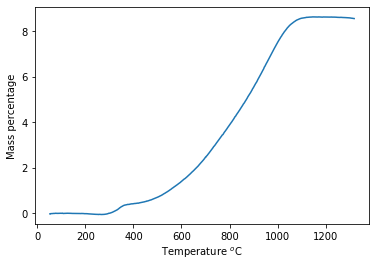
\includegraphics[scale=0.75]{figures/bayesian/1_reaction/EXP/FWC_data.png}
\caption{The FWC curve for a simple experiment where one reaction is occuring.}
\label{fig:FWC_exp}
\end{figure}

We will introduce a variable proposal distribution into our algorithm. The prior information we have in determining the temperature where the reaction rate is maximised, is less precise than our simulated examples. This requires a larger step size initially to explore this space, though we still require a narrower proposal once the chains have converged to efficiently sample the posterior. To implement this our proposal is $N\left(\theta_{t-1},\frac{s}{\sqrt{d}}\right)$, where, $s$ is our fixed proposal standard deviation, and $d$ is our control parameter. We simulate for 20000 iterations total and after we reach 10000 iterations we increase the parameter $d$, narrowing the proposal distribution.\\ 
\begin{figure}[h!]
\centering
\begin{subfigure}{.5\textwidth}
  \centering
  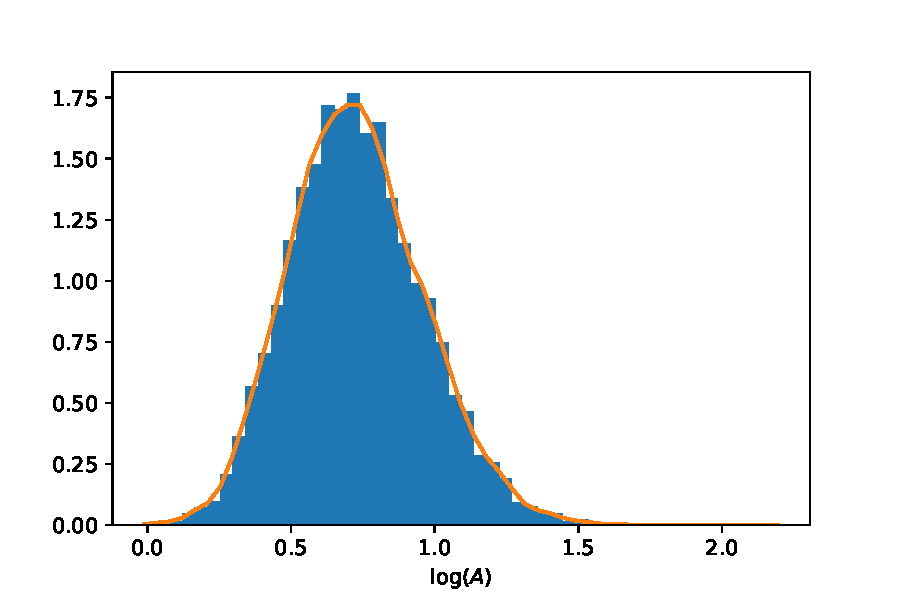
\includegraphics[width=\linewidth]{figures/bayesian/1_reaction/EXP/hist_A.pdf}
  \caption{Histogram of $\tilde{A}$.}
  \label{fig:1EXPA}
\end{subfigure}%
\begin{subfigure}{.5\textwidth}
  \centering
  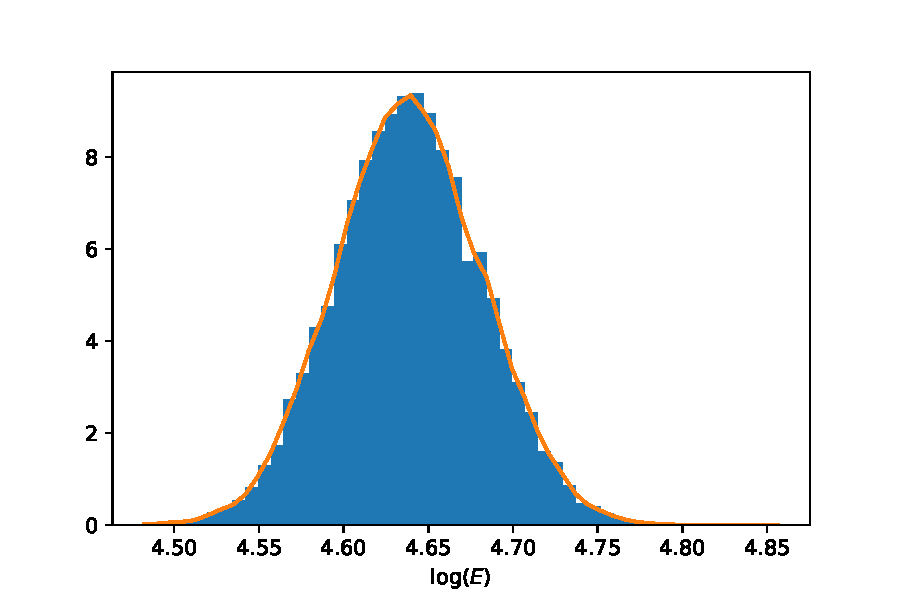
\includegraphics[width=\linewidth]{figures/bayesian/1_reaction/EXP/hist_E.pdf}
  \caption{Histogram of $\tilde{E}$.}
  \label{fig:1EXPE}
\end{subfigure}
\newline
\begin{subfigure}{.5\textwidth}
  \centering
  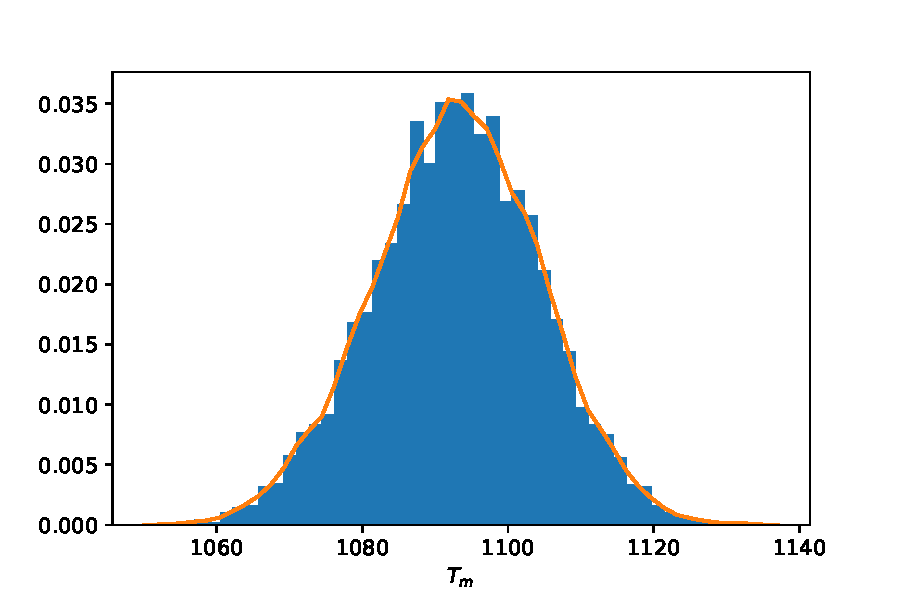
\includegraphics[width=\linewidth]{figures/bayesian/1_reaction/EXP/hist_Tm.pdf}
  \caption{Histogram of $T_m$.}
  \label{fig:1EXPTm}
\end{subfigure}%
\begin{subfigure}{.5\textwidth}
  \centering
  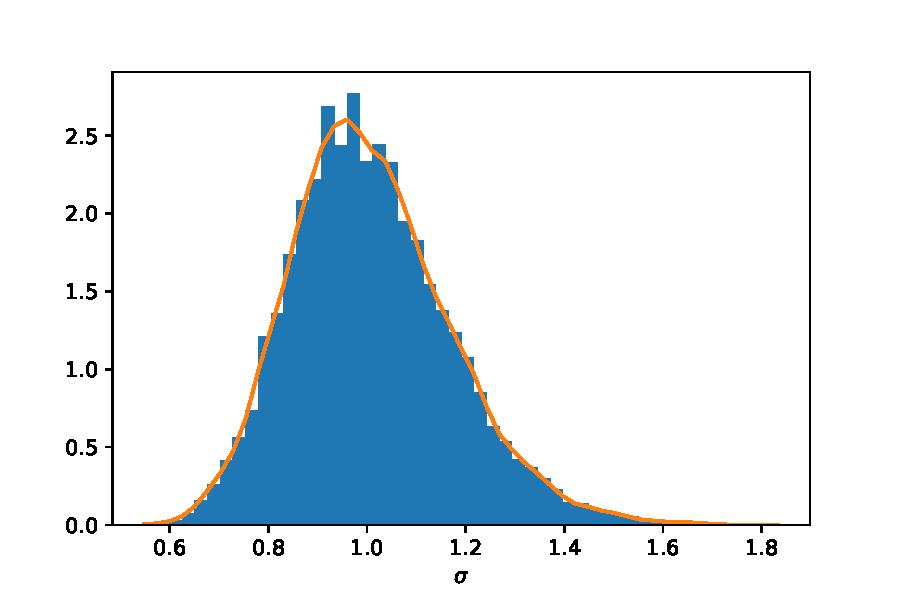
\includegraphics[width=\linewidth]{figures/bayesian/1_reaction/EXP/hist_sigma.pdf}
  \caption{Histogram of $\sigma$.}
  \label{fig:1EXPsigma}
\end{subfigure}
    \caption{Histograms of sampled parameters of the posterior distribution for the experimental data.}%
    \label{fig:EXP1}%s}
\end{figure}%

Figure \ref{fig:EXP1} displays the samples samples from the posterior distribution. This figure indicates that we have a large uncertainty within our parameters. When examining the trace plots in Figure \ref{fig:EXPtrace}, the algorithm behaves as we expect. These trace plots include the first 10000 points sampled which are discarded as burnin. We also observe that the variance in the noise $\sigma$, is much higher than in our simulated examples and is higher than we expect for the experimental data. This suggests that there may be an issue with model misspecification.\\

\begin{figure}[h!]
\centering
\begin{subfigure}{.5\textwidth}
  \centering
  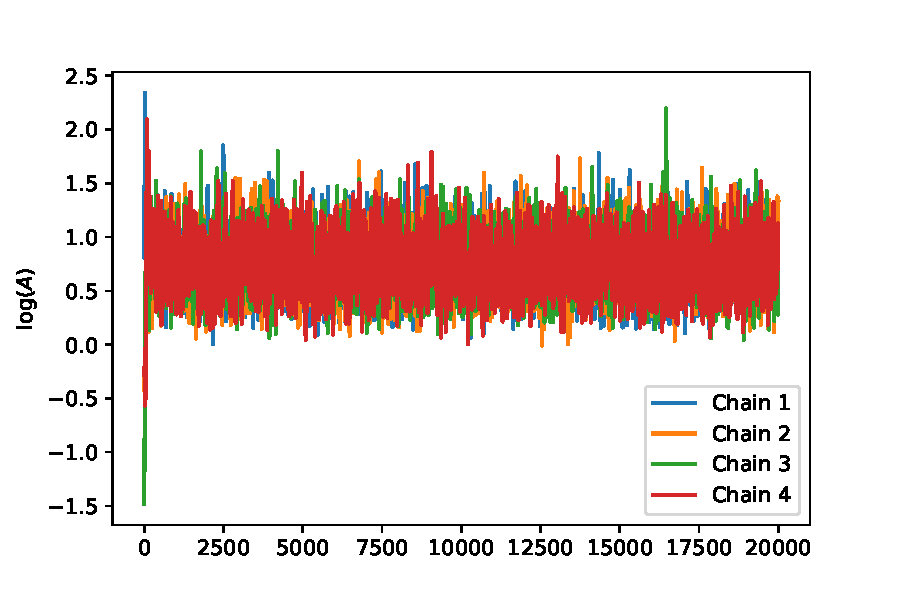
\includegraphics[width=\linewidth]{figures/bayesian/1_reaction/EXP/trace_plot_A.pdf}
  \caption{Trace plot of $\tilde{A}$.}
  \label{fig:1EXPA}
\end{subfigure}%
\begin{subfigure}{.5\textwidth}
  \centering
  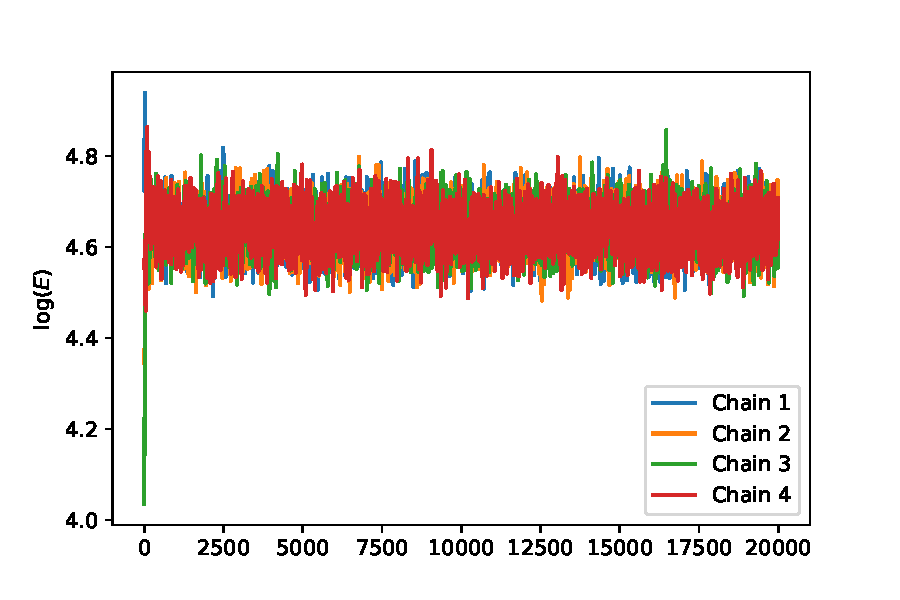
\includegraphics[width=\linewidth]{figures/bayesian/1_reaction/EXP/trace_plot_E.pdf}
  \caption{Trace plot of $\tilde{E}$.}
  \label{fig:1EXPE}
\end{subfigure}
\newline
\begin{subfigure}{.5\textwidth}
  \centering
  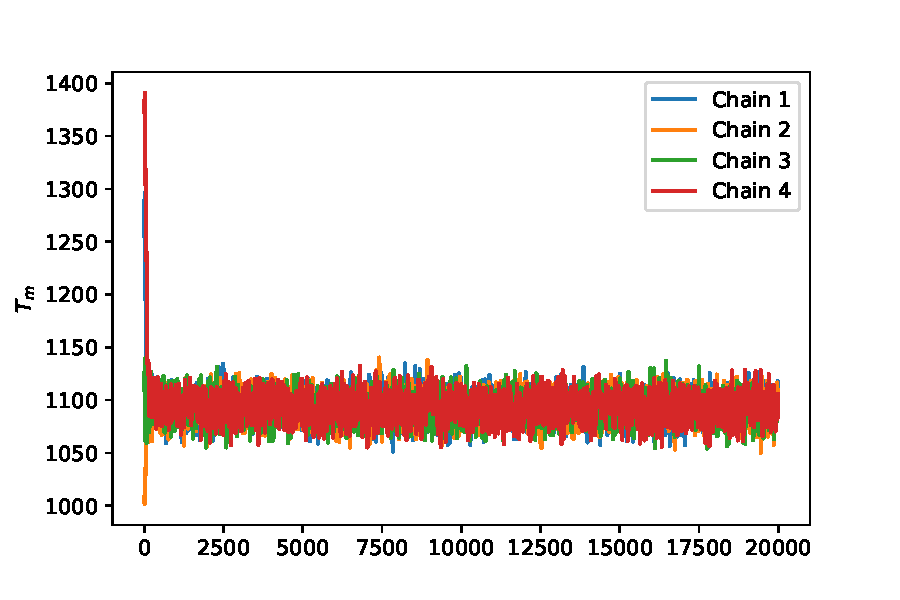
\includegraphics[width=\linewidth]{figures/bayesian/1_reaction/EXP/trace_plot_Tm.pdf}
  \caption{Trace plot of $T_m$.}
  \label{fig:1EXPTm}
\end{subfigure}%
\begin{subfigure}{.5\textwidth}
  \centering
  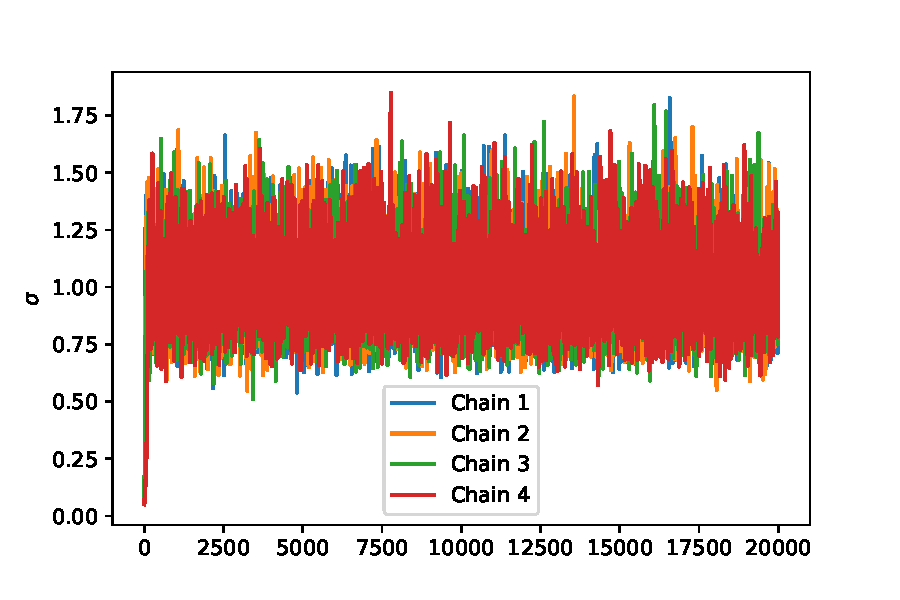
\includegraphics[width=\linewidth]{figures/bayesian/1_reaction/EXP/trace_plot_sigma.pdf}
  \caption{Trace plot of $\sigma$.}
  \label{fig:1EXPsigma}
\end{subfigure}
    \caption{Trace plots for each of the parameters of our MCMC algorithm applied to experimental data.}%
    \label{fig:EXPtrace}%s}
\end{figure}%

To examine the hypothesis that the model doesn't accurately represent the data, we plot some of the sampled curves. We randomly select 10 data points and simualte the experiment and plot them all against the FWC data. What we observe in Figure \ref{fig:comp_exp}, is that the FWC curves find this other mode. What is also worth noting, is that it is difficult to say which curve is a better fit for the data. This is expected through our algorithm. The data has an unusual structure early in the reaction that is likely causing some of these issues.\\

\begin{figure}[h!]
\centering
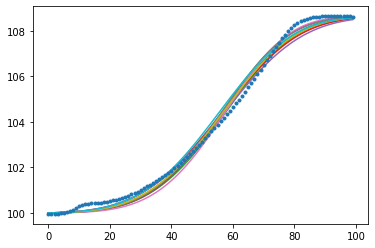
\includegraphics[width=\linewidth]{figures/bayesian/1_reaction/EXP/example_curve.png}
\caption{A random sample of FWC curves against the experimental data.}
\label{fig:comp_exp}
\end{figure}

\begin{figure}[h!]
\centering
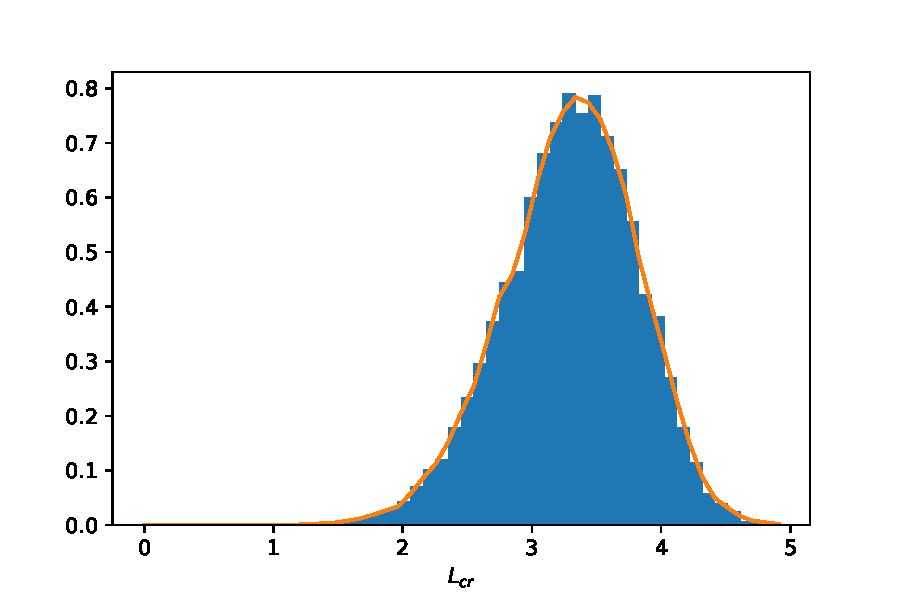
\includegraphics[width=\linewidth]{figures/bayesian/1_reaction/EXP/hist_Lcr.pdf}
\caption{Histogram of the logarithm of the critical length of the stockpile made from the material in the experiment.}
\label{fig:Lcr_exp}
\end{figure}

Persisting with this model we are able to sample from the posterior of the critical length of a stockpile to be built with this material. Figure \ref{fig:Lcr_exp} indicates that the critial length varies over many orders of magnitude. This indicates that using any of these acceptable curves in Figure \ref{fig:comp_exp} in isolation, could provide a poor estimate of the critical length needed for ignition to occur. This highlights the need for consideration of the uncertainty of parameters in assessing models. This analysis indicates that if we wish to approximate the reactions using this model, then we have a large uncertainty within our parameters, and this causes a large uncertainty in the critical length of the stockpiles. To avoid this issue, then we need additional data, or to use an alternative model that can better predict this behaviour. This simple example also indicates the dangers we could face if we use a simple one reaction model as an approximation for more complicated reaction schemes.\\



\section{Two Reactions}
Now that we have an algorithm set up for a single reaction, we extend this to two parallel reactions. For the identifiability of the parameters, we need to ensure the reactions maintain a defined order. Experimentally we can determine which of the two reactions is occurring first, as such the simulations need to reflect this.\\ 

To model the experiment we use the equation defined in equation \ref{FWC_equation},
\begin{equation}
\frac{dM_t}{dt}=w_{c,1}M_1A_1\exp\left(\frac{-E_1}{RT}\right)+w_{c,2}M_2A_2\exp\left(\frac{-E_2}{RT}\right). \label{FWC_equation}
\end{equation}
This equation simplifies down to the equation,
\begin{equation}
M_t=M_{t_0}+w_{c,1}\left(M_1-M_{1_0})\right)+w_{c,2}\left(M_2-M_{2_0})\right),
\end{equation}
where the $0$ subscript denotes the initial masses. The masses, $M_1$ and $M_2$ follow Equation \ref{TGA_system_BI}. We use this weight change equation as it best mimics the experiments that have been conducted. For the statistical model, Equation \ref{FWC_equation}, is used to determine the theoretical solution, which we discretise at given times, $t$. We then add Gaussian noise to our simulated solution.
As our results for the one reaction case indicate that it is better to estimate $T_m$ then we shall explore that parameter space for the two reaction model. We initially consider a scheme with well seperated reactions. The true parameters for our parameter space are defined in table \ref{sim_paras}.\\
For the two reaction models we adjust our algorithm as well. As we introduce more complex behaviour into our model, then efficiency becomes more of an issue. We observed in the one reaction model, that the algorithms can take a significant time to converge. This is computationally inefficient. We also still want our algorthm to have an acceptance rate of approximately $0.234$. As such we divide our algorithm into three stages. Initially we propose from a Gaussian distribution with high variance. In this stage we anticipate the acceptance rate can vary dramatically, but once the optimal node is found, then we will have a low acceptance rate. The intermediate stage has a more narrow proposal distribution where the algorithm refines this node further. The final stage is where we obtain our sample. In this region the algorithm is expected to have converged, so the proposal distribution can be altered to achieve an acceptance rate around the optimal value.\\ 

\begin{table}[h!]
\centering
\begin{tabular}{|c|c|}
\hline
Parameter & value \\ \hline
$E_1$ & $8.6 \times 10^4$ J/mol \\ \hline
$E_2$ & $2.6 \times 10^5$ J/mol\\ \hline
$T_{m,1}$ & 560 K\\ \hline
$T_{m,2}$ & 750 K\\ \hline
$A_1$ & $3.5 \times 10^7 $ m$^3$/kg/s\\ \hline
$A_2$ & $7.1 \times 10^{17} $ m$^3$/kg/s \\ \hline
$\sigma$ & 0.05 \\ \hline
\end{tabular}
\caption{Parameter values for the simulation.}
\label{sim_paras}
\end{table} 

When need to introduce some constraint such that the reactions correspond to the correct portion of the data. Each of the reactions contribute independently to the overall FWC curve. Given that experimentally we can determine which reaction is peaking earlier than our model needs to preserve this. We enforce this constraint through including an informative prior. In our prior we have an additional constraint that $T_{m,1}<T_{m,2}$. We enforce this by using uniform distributions on non-overlapping domains. When the two peaks become closer, we consider a joint prior that enforces this condition.\\

Following Algorithm \ref{Alg:MH}, the samples are presented in Figure \ref{fig:MH3}. These histograms indicate that the chains have converged. The trace plots for these chains also indicate this and can be found in Appendix \ref{App:2_traces}. When we compare these histograms to those in Figure \ref{fig:MH2}, then we observe a similar variances occurring though with two reactions it increases slightly. Interestingly, our sample does not include the true values for $T_{m,2}$ and $\tilde{A_2}$.\\

\begin{figure}[h!]
\centering
\begin{subfigure}{0.5\textwidth}
\centering
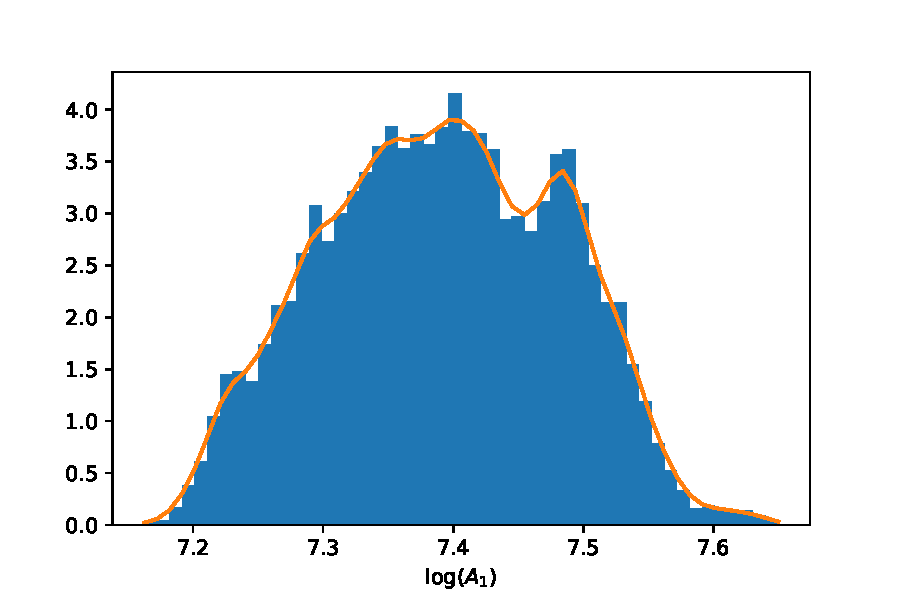
\includegraphics[width=\linewidth]{figures/bayesian/2_reactions/mass/hist_A1.pdf}
\caption{Histogram of $\tilde{A_1}$.}
\label{HistA1}
\end{subfigure}%
\begin{subfigure}{0.5\textwidth}
\centering
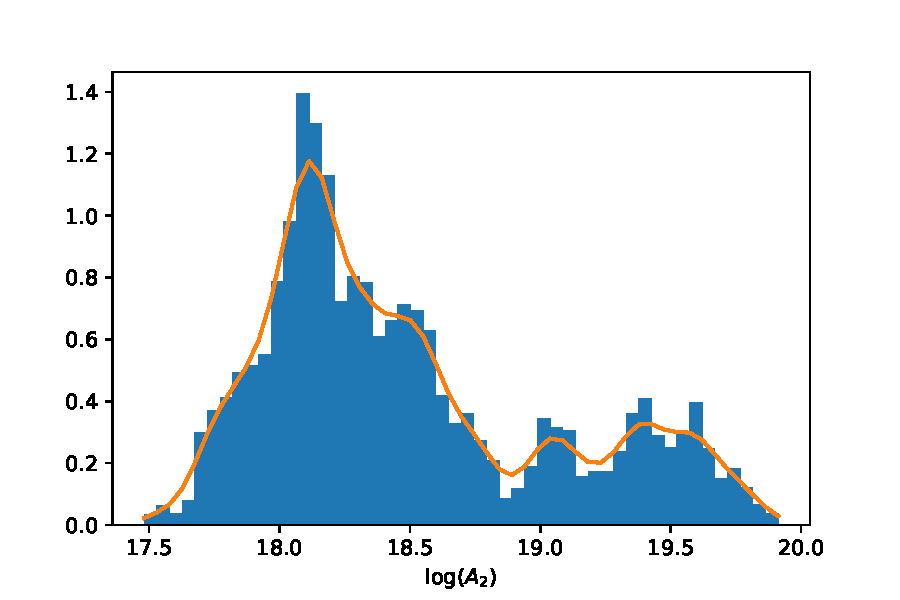
\includegraphics[width=\linewidth]{figures/bayesian/2_reactions/mass/hist_A2.pdf}
\caption{Histogram of $\tilde{A_2}$.}
\label{HistA2}
\end{subfigure}
\newline
\begin{subfigure}{0.5\textwidth}
\centering
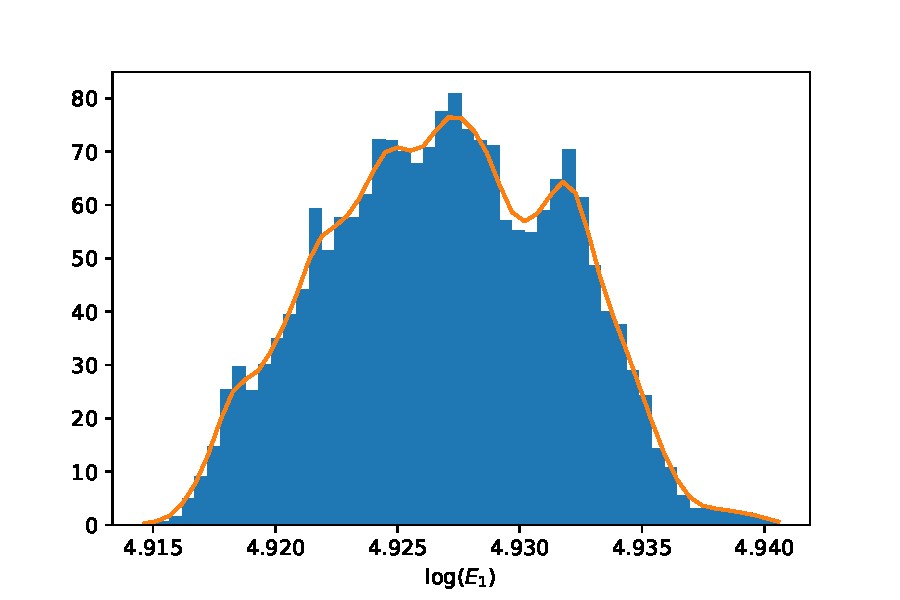
\includegraphics[width=\linewidth]{figures/bayesian/2_reactions/mass/hist_E1.pdf}
\caption{Histogram of $\tilde{E_1}$.}
\label{HistE1}
\end{subfigure}%
\begin{subfigure}{0.5\textwidth}
\centering
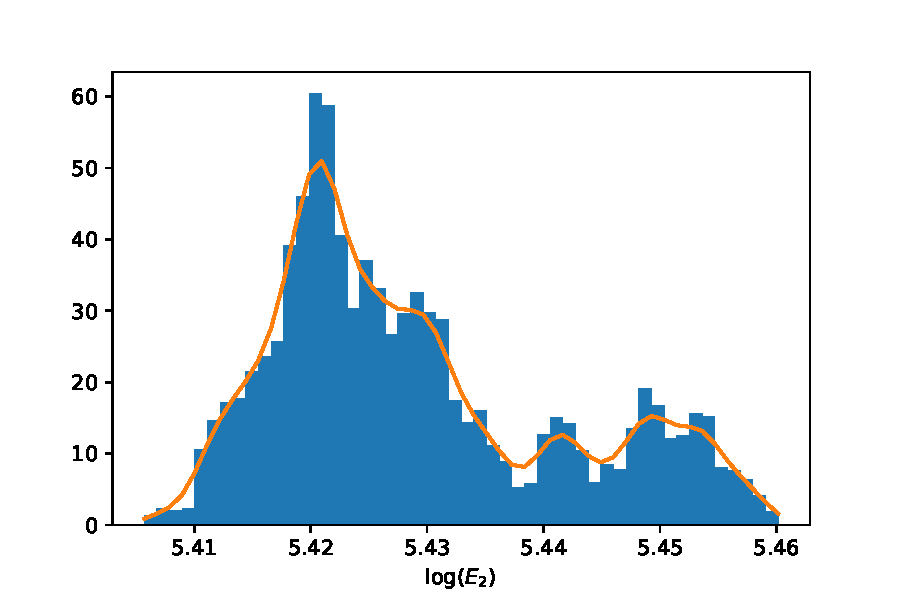
\includegraphics[width=\linewidth]{figures/bayesian/2_reactions/mass/hist_E2.pdf}
\caption{Histogram of $\tilde{E_2}$.}
\label{HistE2}
\end{subfigure}
\newline
\begin{subfigure}{0.5\textwidth}
\centering
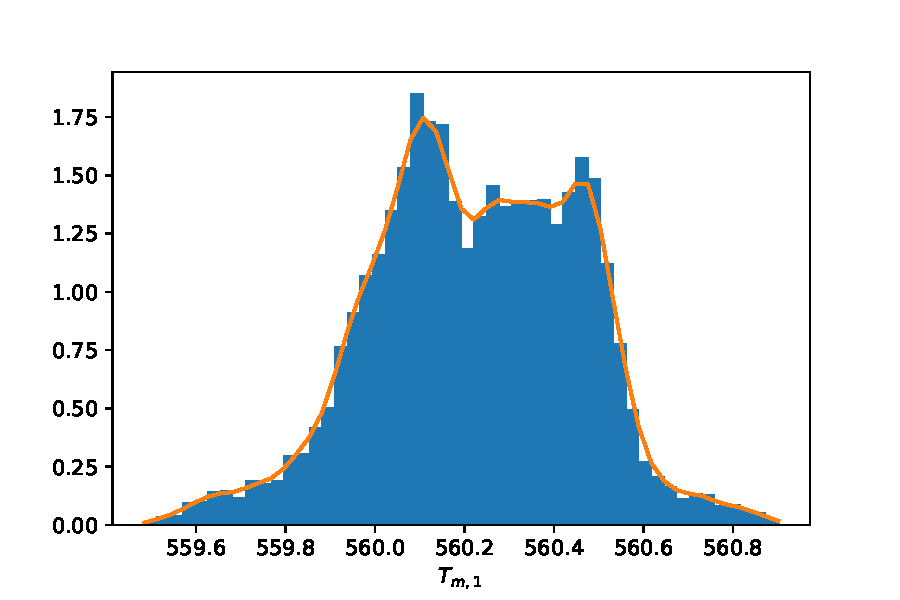
\includegraphics[width=\linewidth]{figures/bayesian/2_reactions/mass/hist_Tm1.pdf}
\caption{Histogram of $T_{m,1}$}
\label{HistTm1}
\end{subfigure}%
\begin{subfigure}{0.5\textwidth}
\centering
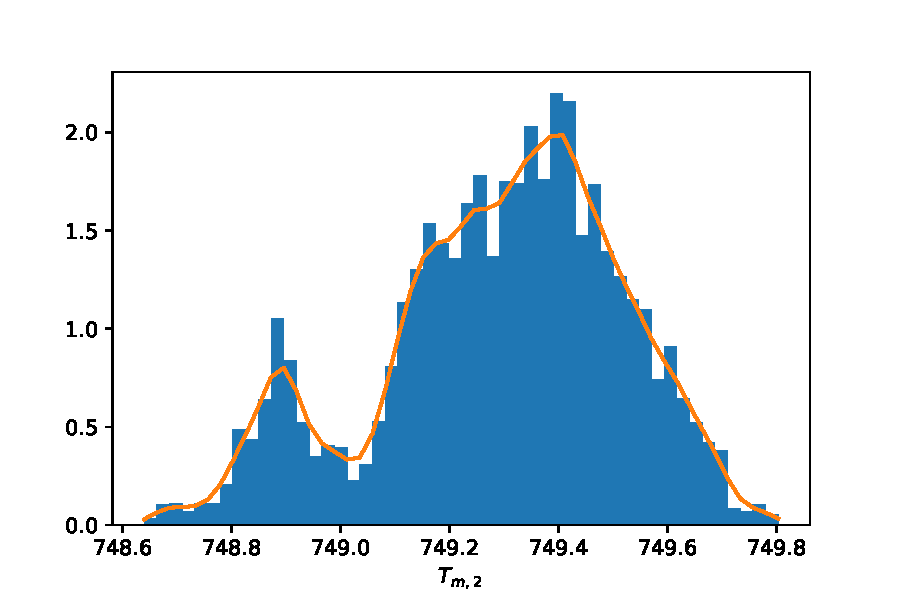
\includegraphics[width=\linewidth]{figures/bayesian/2_reactions/mass/hist_Tm2.pdf}
\caption{Histogram of $T_{m,2}$}
\label{HistTm2}
\end{subfigure}%
\newline
\begin{subfigure}{0.5\textwidth}
\centering
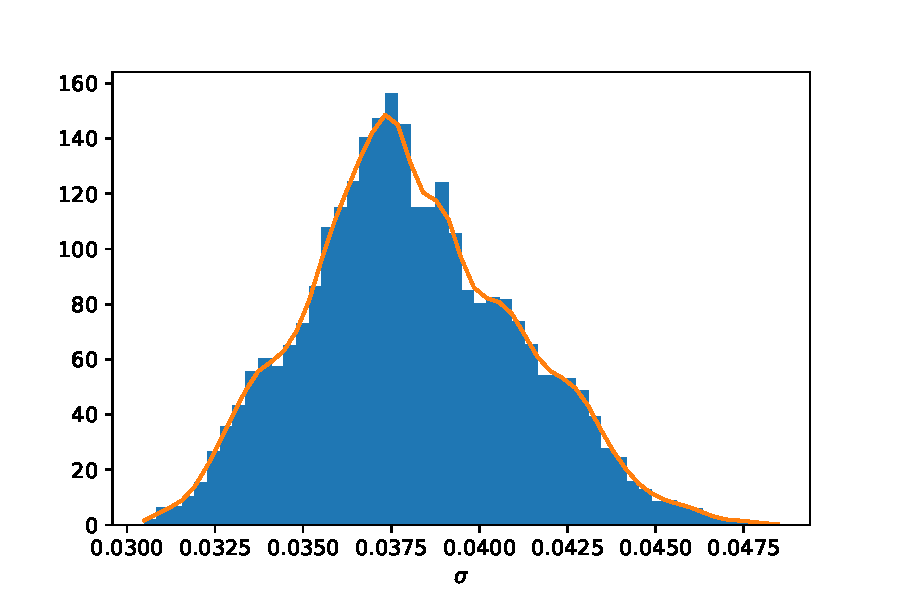
\includegraphics[width=\linewidth]{figures/bayesian/2_reactions/mass/hist_sigma.pdf}
\caption{Histogram of $\sigma$}
\label{Histsigma2}
\end{subfigure}%
\caption{Output from the Metropolis-Hastings for an experiment with two reactions.}
\label{fig:MH3}
\end{figure}

\begin{figure}[h!]
\centering
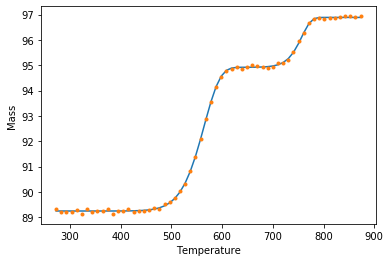
\includegraphics[scale=0.7]{figures/bayesian/2_reactions/mass/Example_FWC.png}
\caption{Example of a FWC change curve with two seperated equations.}
\label{fig:FWC_EX2}
\end{figure}

Figure \ref{fig:FWC_EX2}, plots an example of the FWC curve, generated using one of the sampled points and compares this to the the noisy data. This highlights an issue that may be arising from a lack of datapoints. There are minimal datapoints where the seond reaction is occurring, and this may contribute to why the sample obtained does not include the true parameters. Figure \ref{fig:FWC_EX2} clearly indicates that the sampled parameters still provide a good fit for the data.\\

This data is very simple, with well separated reactions. This indicates that our algorithm is useful to estimate these parameters for well seperated reactions. In the experimental data we use, the reactions are not well seperated. We simulate some new data using altered parameters. We change the parameters $T_{m,1}$ and $T_{m,2}$ such that, $T_{m,1}=620$ and $T_{m,2}=700$. Given these values are much closer, from the data itself it is harder to distinguish where the two peaks are. The non-overlapping uniform prior will not be useful in this scenario. Instead we consider a uniform prior over the region, $550<T_{m,1}<T_{m,2}<750$. This prior enforces our identifiability constraint, $T_{m,1}<T_{m,2}$, and bounds each value. It is possible to have other priors that fit these constraints, though we use this prior for its simplicity.\\

Conducting the inference we obtain the samples displayed in Figure \ref{fig:MH4}. In these samples we correctly obtain the true parameter values for each parameter. With the additional data points we do not have the issue before where the true parameter was outside our sampled values. We are able to successfully implement our algorithm to estimate the parameters with two reactions. It is reasonable to expect that we can apply this algorithm to include additional reactions. There is limitations that the reactions will have to be seperated in such a way that we can impose useful prior information.

\begin{figure}[h!]
\centering
\begin{subfigure}{0.5\textwidth}
\centering
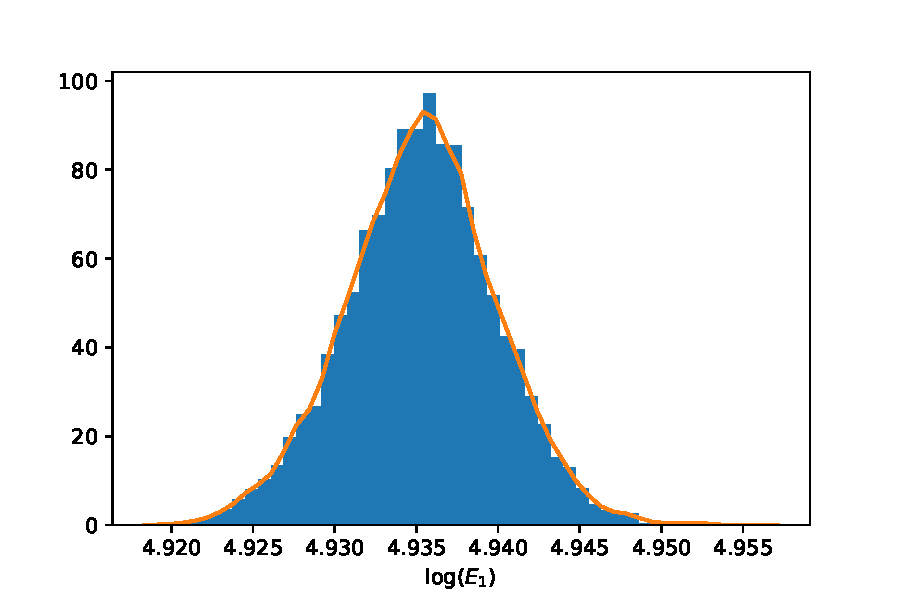
\includegraphics[width=\linewidth]{figures/bayesian/2_reactions/mass_close/hist_E1.pdf}
\caption{Histogram of $\tilde{E_1}$.}
\label{HistE12}
\end{subfigure}%
\begin{subfigure}{0.5\textwidth}
\centering
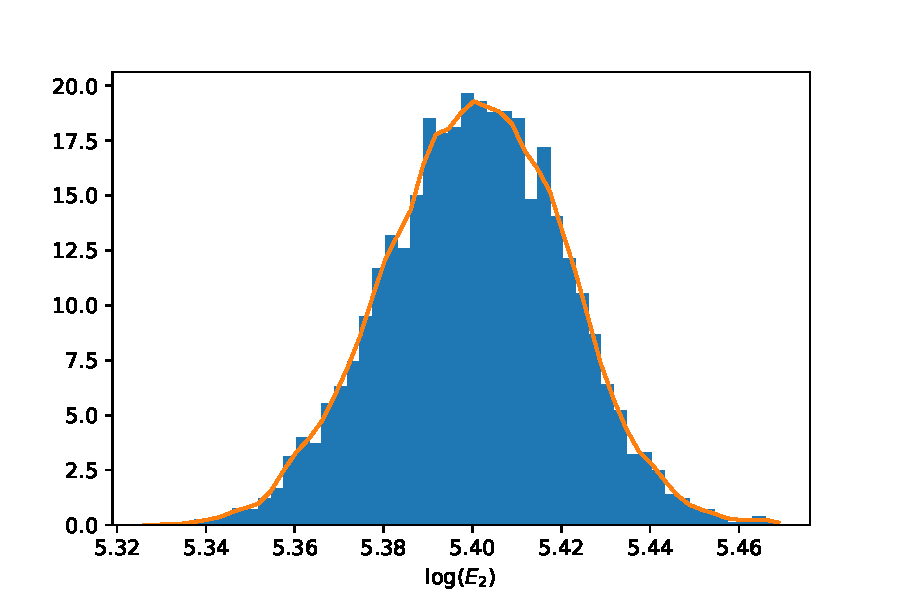
\includegraphics[width=\linewidth]{figures/bayesian/2_reactions/mass_close/hist_E2.pdf}
\caption{Histogram of $\tilde{E_2}$.}
\label{HistE22}
\end{subfigure}
\newline
\begin{subfigure}{0.5\textwidth}
\centering
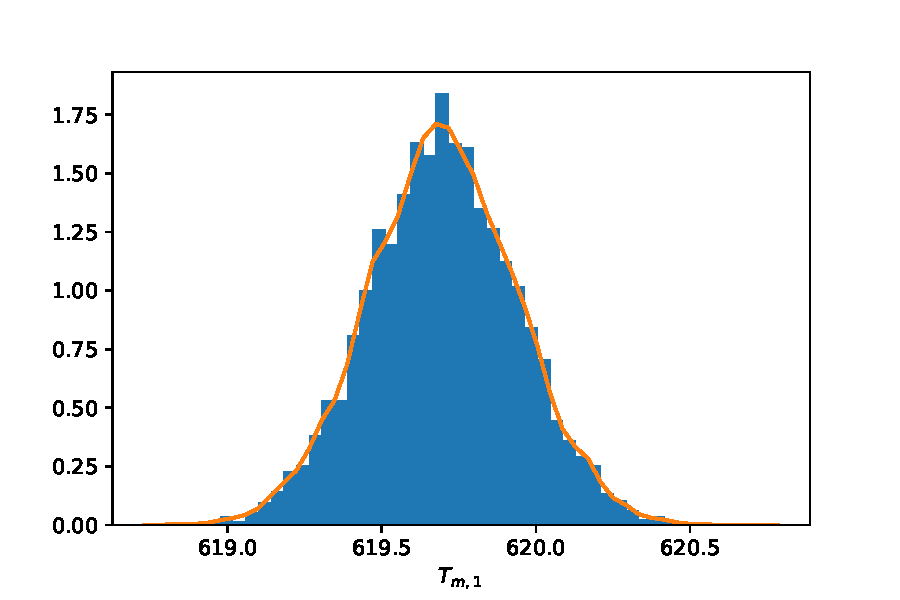
\includegraphics[width=\linewidth]{figures/bayesian/2_reactions/mass_close/hist_Tm1.pdf}
\caption{Histogram of $T_{m,1}$}
\label{HistTm12}
\end{subfigure}%
\begin{subfigure}{0.5\textwidth}
\centering
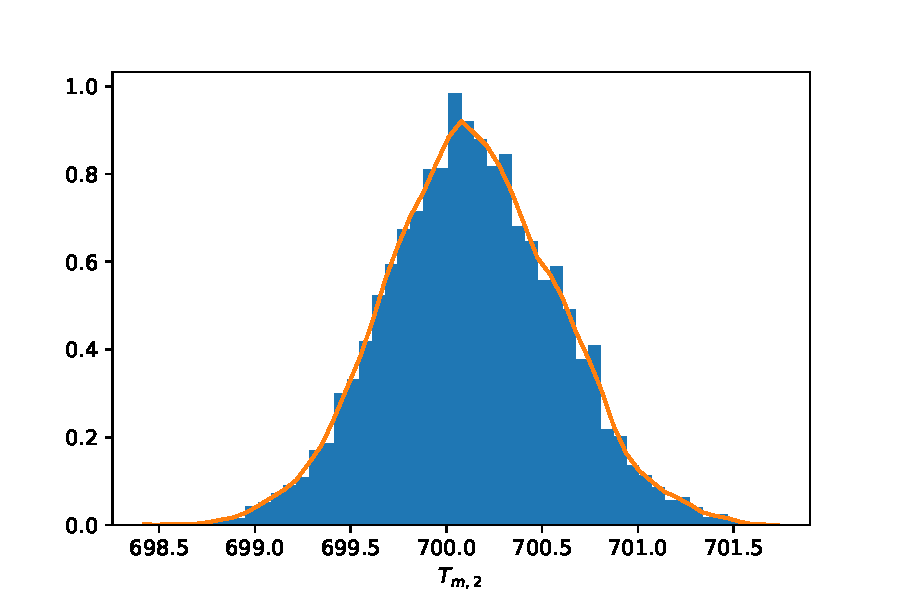
\includegraphics[width=\linewidth]{figures/bayesian/2_reactions/mass_close/hist_Tm2.pdf}
\caption{Histogram of $T_{m,2}$}
\label{HistTm22}
\end{subfigure}%
\newline
\begin{subfigure}{0.5\textwidth}
\centering
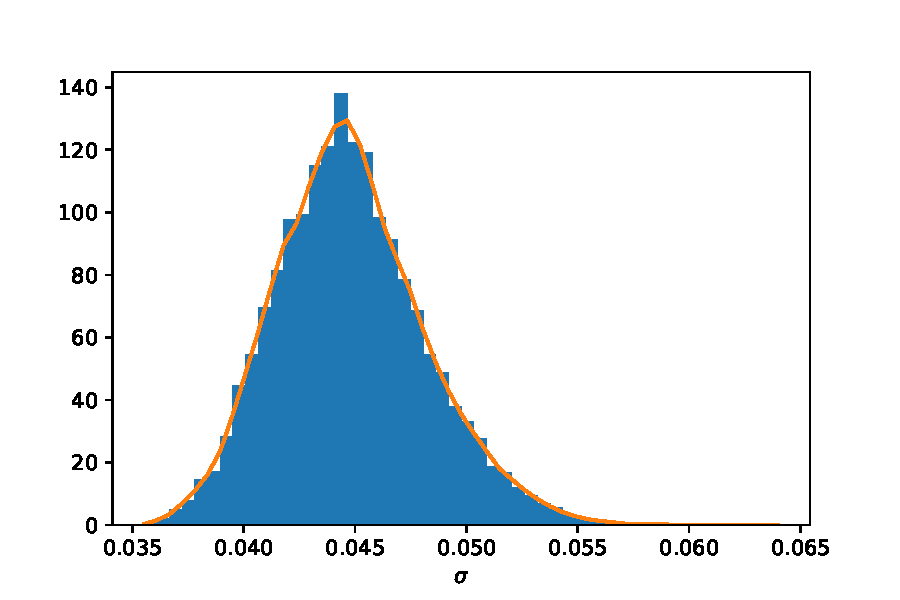
\includegraphics[width=\linewidth]{figures/bayesian/2_reactions/mass_close/hist_sigma.pdf}
\caption{Histogram of $\sigma$}
\label{Histsigma22}
\end{subfigure}%
\caption{Output from the Metropolis-Hastings for an experiment with two reactions, close together.}
\label{fig:MH4}
\end{figure}


\subsubsection{Multi-Modality}
The algorithm that we are using is not always work without issues. We found that when using a different model, our posterior distribution identified different modes. We use the model,
\begin{align*}
\frac{dM_1}{dt}&=-M_1OA_1\exp\left(\frac{-E_1}{RT}\right), \\
\frac{dM_2}{dt}&=-M_2^3OA_2\exp\left(\frac{-E_2}{RT}\right), \\ 
\frac{dT}{dt}&=\alpha, %\label{TGA_system2_BI}.
\end{align*}
This model is for a third order Arrhenious reaction for the second reaction rather than a first order. In future work we may consider different models, though our current analysis focuses upon first order reactions. \\
When using higher order reactions Equation \ref{eqkis}, becomes,
\begin{equation}
A\exp\left(\frac{-E}{RT_m}\right)nM_m^{n-1}=\frac{E}{RT_m^2}\frac{dT}{dt}, \label{eqkis2}
\end{equation}
where $n$, is the reaction order and $M_m$ is the mass when the reaction rate is maximised. We cannot use this equation to propose new values of $A$, as the mass term $M_m$ is dependant upon the parameters $(A,E,T_m)$. This yields an implicitly defined function for $A$, which is unlikely to yield any significant gains in computation speed. We can still use the Equation \ref{eqkis} as a means to propose new $A$ values, though the $T_m$ parameter in this case will not have the same meaning. This still reduces some of the issues we found when using the parameters $(A,E)$, though the prior information is not as useful.\\

We produce a simulated sample using the same parameters specified in Table \ref{sim_paras}. These parameters use Equation \ref{eqkis} to relate the Pre-exponential factor to the Activation Energy, and temperature $T_m$. This simulated data is displayed in Figure \ref{fig:modal_sim}. We observe that the second reaction rate is not maximised at the $T_m$ value stated in Table \ref{sim_paras}. This also highlights some issues with identifiability of the two reactions. We can no longer define the order of the reactions using this $T_m$ parameter.
 
\begin{figure}[h!]
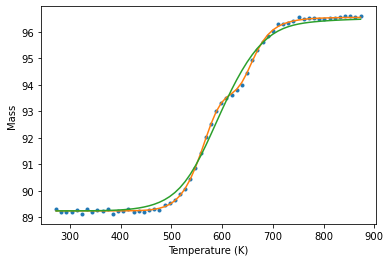
\includegraphics[scale=1]{figures/bayesian/2_reactions/TGA_comparison.png}
\caption{This figure needs to be updated.}
\label{fig:modal_sim}
\end{figure}
%
%After running the MCMC algorithm we observed that it does not always converge. Figure \ref{comparison} depicts the estimated mass of the sample for different sampled parameters. We observe that in some cases, the chains appear to be blurring the reactions together. It appears as though the MCMC algorithm is sampling around a local optimum value rather than the true optimal value.\\

We examine the bahaviour of the four chains as they move through the parameter sapce. Figure \ref{fig:walks} indicates that the value that the mode each chain samples around is dependant upon the initial proposal for the sampling algorithm. We observe two chains (red and orange) sample the true parameters in our model, whilst the other chains sample a much larger region. \\

\begin{figure}[h!]
\centering
\begin{subfigure}{.5\textwidth}
  \centering
  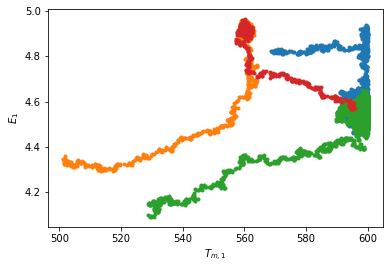
\includegraphics[width=\linewidth]{figures/bayesian/2_reactions/E1vsTm1.png}
  \caption{Random walks for the first reaction.}
  \label{fig:subwalk1}
\end{subfigure}%
\begin{subfigure}{.5\textwidth}
  \centering
  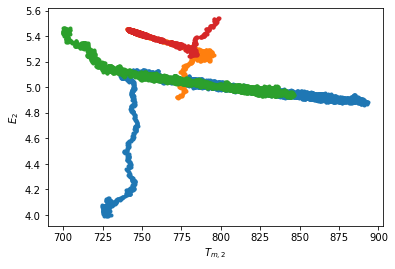
\includegraphics[width=\linewidth]{figures/bayesian/2_reactions/E2vsTm2.png}
  \caption{Random walks for the second reaction.}
  \label{fig:subwalk2}
\end{subfigure}%
\caption{Random walks for the maximal temperature and activation energy for the two reactions in a simulated system.}
\label{fig:walks}
\end{figure}

We claimed earlier that by proposing new values of $T_m$, we are still able to eliminate some of the issues with proposing the parameters,$(A,E)$. Figure \ref{fig:modal_sample} indicates that the sample from the chains that converged around the true parameters are uncorrelated. This indicates that although the parameter $T_m$ has lost its physical interpretation, the parameters $(A,E)$ are still near correlated along the cruve in \ref{eqkis}.\\

\begin{figure}[h!]
\centering
\begin{subfigure}{.5\textwidth}
  \centering
  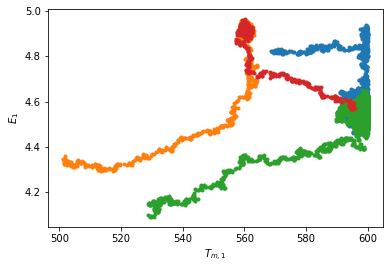
\includegraphics[width=\linewidth]{figures/bayesian/2_reactions/E1vsTm1.png}
  \caption{Random walks for the first reaction.}
  \label{fig:subwalk1}
\end{subfigure}%
\begin{subfigure}{.5\textwidth}
  \centering
  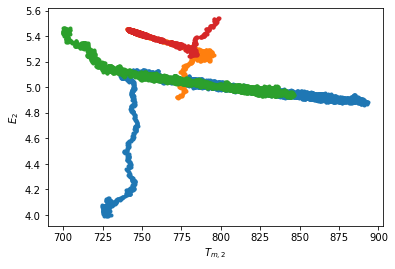
\includegraphics[width=\linewidth]{figures/bayesian/2_reactions/E2vsTm2.png}
  \caption{Random walks for the second reaction.}
  \label{fig:subwalk2}
\end{subfigure}%
\caption{Samples of the converged chain for the maximal temperature and activation energy for the two reactions in a simulated system.}
\label{fig:modal_sample}
\end{figure}

\begin{figure}[h!]
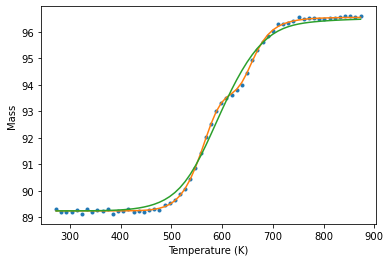
\includegraphics[scale=1]{figures/bayesian/2_reactions/TGA_comparison.png}
\caption{Comparison of two sampled parameter values for the two reaction case.}
\label{comparison}
\end{figure}

Figure \ref{comparison} plots example FWC curves within each mode. We see that mode 1 is able to approximate the data well whilst mode 2, seems to approximate the two reactions by a single reaction. This could potentially arise from the fact we are not using good information about the $T_m$ parameter. Implementing this in the way we have, could disrupt the algorithms ability to identify the reaction order and this results in this mode occuring. The key takeaway frm this is when we consider the experimental data, this issue may occur. The multi-modality is something we need to take into consideration.

\subsection{DSC}
With the issues of multi-modality we opt to use more of the experimental data. We include the addition of the DSC data into our simulations. The contribtion of each reaction to the DSC data is proportional to the reaction rate. By adding the DSC data, we are effectively adding information about the gradients of the FWC into our algorithm. This will ensure that what we observed in Figure \ref{comparison}, where the reactions combine, have a significantly lower likelihood. The adjusted algorithm is displayed in Algorithm \ref{Alg:MH_DSC}. It is important to note that the DSC data is calculated based off the mass of each substance from our solution vector.\\

Utilising the DSC data introduce s two new variables into the equation, $Q_1$ and $Q_2$. These denote the heat given by the reaction. We deal with the parameters in two ways. We can pre-assign the parameter values, or we can estimate these parameters through the MCMC algorithm. The results presented in Figure \ref{fig:DSC_4hist} use preassigned values. For the experimental data we estimate these parameters as they can be used to provide a better fit for the data. If there are multiple reactions occurring that mimic a single reaction. Estimating the heat of reaction parameters allows us to capture this information and characterise the heat in terms of a single reaction. This provides more valuable information when translating the theory across to the stockpiles where the temperature at each point of the pile is the key piece of information we are interested in.\\
We also have to consider the error for each of the mass and DSC data. We want to ensure that our algorithm isn't favouring one set of data over the other. We address this in our algorithm by setting the noise parameters so that the relative variances scale. The alternative is to have separate noise parameters to estimate. We have opted to include separate noise parameters, and then use the prior to force the variances to scale in some degree.\\

\begin{algorithm}[H]
\SetAlgoLined
\KwResult{}
 Initialise $\theta_0$ by sampling from the prior\;
 \For{$t=0:$sample\_size}{
  Sample $\theta ^*~ \sim ~ Q(\theta^*|\theta)$ \;
  Evaluate $\textbf{F}_\tau(\theta^*)$ \# solve differential equation\;
  Evaluate $\textbf{D}_\tau(\theta^*)$ \# calculate the DSC\;
  Set $\alpha = \frac{P(\textbf{y}|\theta^*)Q(\theta_{t-1}|\theta^*)P(\theta^*)}{P(\textbf{y}|\theta)Q(\theta^*|\theta_{t-1})P(\theta_{t-1})}$\;
  Sample $b ~ \sim ~U(0,1)$\;
  \eIf{$\alpha>b$}{
   Set $\theta_t=\theta^*$} {
   Set $\theta_t=\theta_{t-1}$
   }
 }
 \caption{Metropolis Hastings Algorithm for determining the posterior distribution with FWC and DSC data.}
 \label{Alg:MH_DSC}
\end{algorithm}

With this algorithm we now consider two cases; Fixed heat parameters, where we prescribe the values of $Q_1$ and $Q_2$, and our Inferred Parameters, where we conduct inference on the parameters $Q_1$ and $Q_2$.  
\subsubsection{Fixed Heat Parameters}
The first case is where we consider fixed heat parameters. This is a simple case where we can examine the effects of the addition of the DSC data without increasing the dimension of our problem. In a practical application we may not be able to prescribe these heat parameters and this limits the practical implementation of this method. Figure \ref{fig:DSC_4hist} displays the posterior distributions obtained from the simulated data. When we compare that to the data posterior samples in Figure \ref{fig:MH4}, then we observe that the histograms are much narrower. The samples in Figure \ref{fig:DSC_4hist} still contain the true values as well. With adding the DSC data into the simulations we have decreased the uncertainty in the posterior distributions.\\
%
\begin{figure}[h!]
\centering
\begin{subfigure}{.5\textwidth}
  \centering
  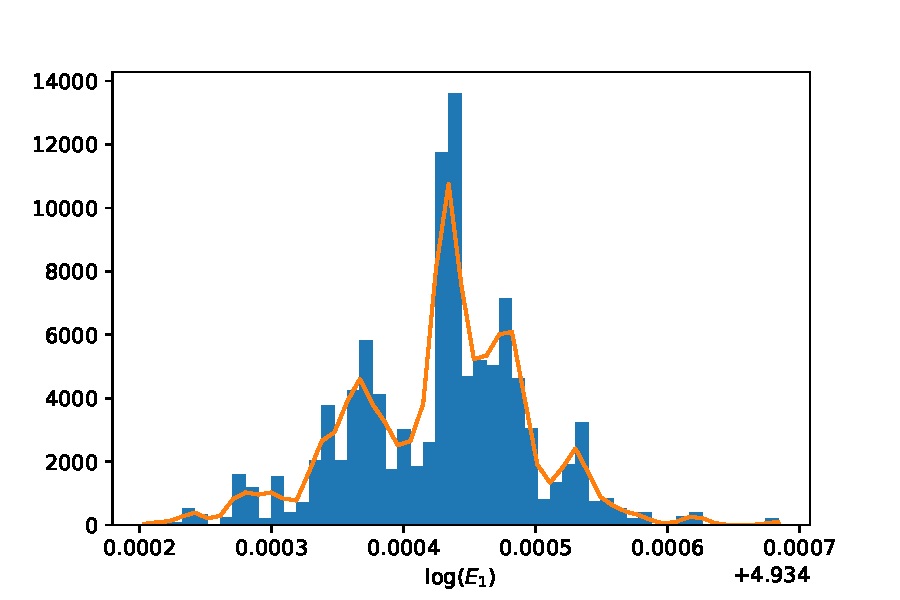
\includegraphics[width=\linewidth]{figures/bayesian/SIM/hist_E1.pdf}  \caption{Distribution of $\log E_1$.}
  \label{fig:subhistE1}
\end{subfigure}%
\begin{subfigure}{.5\textwidth}
  \centering
  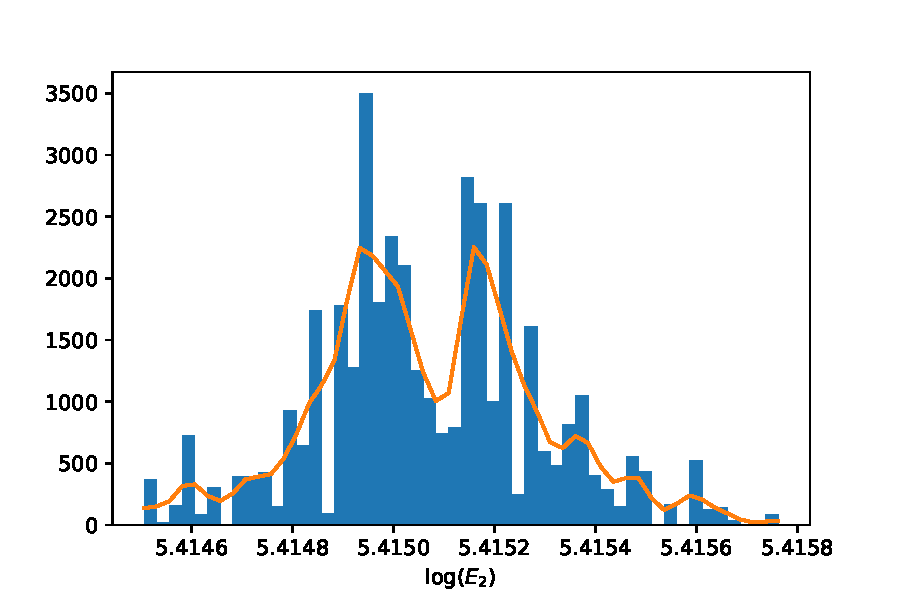
\includegraphics[width=\linewidth]{figures/bayesian/SIM/hist_E2.pdf}
  \caption{Distribution of $\log E_2$.}
  \label{fig:subhistE2}
\end{subfigure}
\newline
\begin{subfigure}{.5\textwidth}
  \centering
  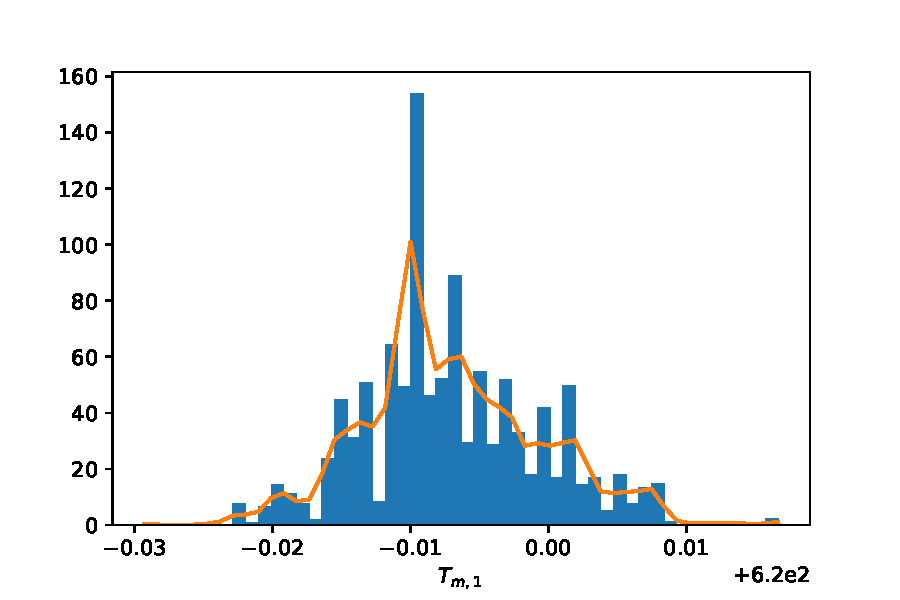
\includegraphics[width=\linewidth]{figures/bayesian/SIM/hist_Tm1.pdf}
  \caption{Distribution of $T_{m,1}$.}
  \label{fig:subhistTm1}
\end{subfigure}%
\begin{subfigure}{.5\textwidth}
  \centering
  \includegraphics[width=\linewidth]{figures/bayesian/SIM/hist_Tm2.pdf}
  \caption{Distribution of $T_{m,2}$.}
  \label{fig:subhistTm2}
\end{subfigure}
\newline
\begin{subfigure}{.5\textwidth}
  \centering
  \includegraphics[width=\linewidth]{figures/bayesian/SIM/hist_sigma.pdf}
  \caption{Distribution of $\sigma$.}
  \label{fig:subhistTm1}
\end{subfigure}%
%\begin{subfigure}{.5\textwidth}
%  \centering
%  \includegraphics[width=\linewidth]{figures/bayesian/SIM/hist_sigmaD.pdf}
%  \caption{Distribution of $\sigma_D$.}
%  \label{fig:subhistTm2}
%\end{subfigure}
    \caption{Distributions of the estimated parameters.}%
    \label{fig:DSC_4hist}%s}
\end{figure}%

\subsubsection{Inferred Parameter}
The alternative method for including these heat parameters is to conduct inference on them. This setting is more useful for practical problems where these parameters are unknown. As mention before that introducing new parameters into the inference increases the dimensionality of the problem and could lead to more multi-modal behaviour. The samples from the posterior distribution are displayed in Figure \ref{fig:DSC_8hist}

\begin{figure}[h!]
\centering
\begin{subfigure}{.5\textwidth}
  \centering
  \includegraphics[width=\linewidth]{figures/bayesian/SIM_Q/hist_E1.pdf}  \caption{Distribution of $\log E_1$.}
  \label{fig:subhistE1}
\end{subfigure}%
\begin{subfigure}{.5\textwidth}
  \centering
  \includegraphics[width=\linewidth]{figures/bayesian/SIM_Q/hist_E2.pdf}
  \caption{Distribution of $\log E_2$.}
  \label{fig:subhistE2}
\end{subfigure}
\newline
\begin{subfigure}{.5\textwidth}
  \centering
  \includegraphics[width=\linewidth]{figures/bayesian/SIM_Q/hist_Tm1.pdf}
  \caption{Distribution of $T_{m,1}$.}
  \label{fig:subhistTm1}
\end{subfigure}%
\begin{subfigure}{.5\textwidth}
  \centering
  \includegraphics[width=\linewidth]{figures/bayesian/SIM_Q/hist_Tm2.pdf}
  \caption{Distribution of $T_{m,2}$.}
  \label{fig:subhistTm2}
\end{subfigure}
\newline
\begin{subfigure}{.5\textwidth}
  \centering
  \includegraphics[width=\linewidth]{figures/bayesian/SIM_Q/hist_Q1.pdf}
  \caption{Distribution of $Q_{1}$.}
  \label{fig:subhistTm1}
\end{subfigure}%
\begin{subfigure}{.5\textwidth}
  \centering
  \includegraphics[width=\linewidth]{figures/bayesian/SIM_Q/hist_Q2.pdf}
  \caption{Distribution of $Q_{2}$.}
  \label{fig:subhistTm2}
\end{subfigure}
\newline
\begin{subfigure}{.5\textwidth}
  \centering
  \includegraphics[width=\linewidth]{figures/bayesian/SIM_Q/hist_sigma.pdf}
  \caption{Distribution of $\sigma$.}
  \label{fig:subhistTm1}
\end{subfigure}%
\begin{subfigure}{.5\textwidth}
  \centering
  \includegraphics[width=\linewidth]{figures/bayesian/SIM_Q/hist_sigmaD.pdf}
  \caption{Distribution of $\sigma_D$.}
  \label{fig:subhistTm2}
\end{subfigure}
    \caption{Distributions of the estimated parameters.}%
    \label{fig:DSC_8hist}%s}
\end{figure}%

When we compare the histograms in Figure \ref{fig:DSC_8hist} to those in Figure \ref{fig:DSC_4hist}, then we observe that the variance of the posterior distributions is much greater when we infer the heat parameters. This is not a surprising result as we are adding in more unknowns into the model. Figure \ref{fig:DSC_8hist} also indicates that we have successfully captured the true parameters within our posterior distrbutions. (Currently I have used the old values in the script and didn't update them so they are different).



\section{Application to Experimental Data}
Now that we have established the algorithm is able to infer information about our parameters in our simulated examples we can apply this to experimental data. The experimental data is more complex and there is also the case where we can have model misspecification. We persist with the model,
\begin{align}
\frac{dM_1}{dt}&=M_1A_1\exp\left(\frac{-E_1}{RT}\right),\\
\frac{dM_2}{dt}&=M_2A_2\exp\left(\frac{-E_2}{RT}\right),\\
\frac{dT}{dt}&=\alpha,\\
\frac{dM_t}{dt}&=w_{c,1}M_1A_1\exp\left(\frac{-E_1}{RT}\right)+w_{c,2}M_2A_2\exp\left(\frac{-E_2}{RT}\right), \\
H&=Q_1M_1A_1\exp\left(\frac{-E_1}{RT}\right)+Q_2M_2A_2\exp\left(\frac{-E_2}{RT}\right),\\
\end{align}
that we derived the respective parts for in Section \ref{SEC:TGA}. This first order Arrhenious equation model will also link into our large stockpile models and thus it is imperative that we conduct inference on these parameters. The experimental data is obtained from the work done by Longbottom et al \cite{Ray19} and displayed in Figure \ref{fig:EXP_data}.\\ 

\begin{figure}[h!]
\centering
\begin{subfigure}{.5\textwidth}
  \centering
  \includegraphics[width=\linewidth]{figures/TGA_exp.jpg}  
  \caption{Fractional weight change curve.}
  \label{fig:exp_fwc}
\end{subfigure}%
\begin{subfigure}{.5\textwidth}
  \centering
  \includegraphics[width=\linewidth]{figures/DSC_exp.jpg}
  \caption{Differential Scanning Calorimetry data.}
  \label{fig:exp_DSC}
\end{subfigure}
\label{fig:EXP_data}
\caption{Experimental data on the Filter cake \cite{Ray19}.}
\end{figure} 

This data includes all the reactions that are occuring within the stockpile. If we were to use all of the data we would need at least 5 reactions, of which many are unlikely to be identified through experimentation. We focus our analysis on the critical region from $200^oC$ to $500^oC$. This region was identified by Longbottom et al. \cite{Ray19} as the region where the reaction that are the primary drivers of selfheating are occuring. The restricted data is displayed in Figure \ref{fig:Res_data}, for clarity.\\

\begin{figure}[h!]
\centering
\begin{subfigure}{.5\textwidth}
  \centering
  \includegraphics[width=\linewidth]{figures/FWC.png}  
  \caption{Restricted FWC curve.}
\end{subfigure}%
\begin{subfigure}{.5\textwidth}
  \centering
  \includegraphics[width=\linewidth]{figures/Dsc.png}
  \caption{Restricted DSC data.}
  \label{fig:res_DSC}
\end{subfigure}
\label{fig:Res_data}
\caption{Experimental data on the Filter cake restricted to the critical region \cite{Ray19}.}
\end{figure}

When we are applying the algorithm to experimental data it is important to consider the effect of the parameters we aren't conducting the inference on. The specific parameters of interest are the initial mass concentrations, denoted $M_{1,0}$ and $M_{2,0}$, and the weight change constants, $w_{c,1}$ and $w_{c,2}$. We determine the weight change constants by prescribing the reaction scheme, 
\begin{align*}
3\text{Fe}+2\text{O}_2 &\rightarrow \text{Fe}_3\text{O}_4, \\
6\text{FeO}+\text{O}_2 &\rightarrow 2\text{Fe}_3\text{O}_4, \\
\end{align*}
stated in Section \ref{Sec:stockpile}. Using this reaction scheme we can determine the amount of mass that is added to the sample per gram of Iron and W\"ustite consumed. These weight change constants are stated in nomenclature.\\
The initial masses are more challenging. The filter cake is known to be highly heterogeneous and as a result the initial masses in the sample can vary from the measured values determined by Longbottom et al \cite{Ray19}. It is important to have accurate estimates for these parameters as they can introduce error into the model and the estimates of the reaction parameters can have an unkown bias. We control for this by ensuring that the simulated sample mass at the beginning and end of the critical region closely match the sample mass in the experiment. To calculate this we impose an assumption that there is negligible mass change from these reactions outside of this region. Under this assumption we also assume that the moistureless mass is the minimum sample mass. This results in the equation,
\begin{equation}
M_{1,0}w_{c,1}+M{2,0}w_{c,2}=M_{t,0}-M_{t,f}. \label{eq:constraint}
\end{equation} 
To determine the initial concentrations we minimise the distance, $d=\lvert \left(M_{1,0}-\tilde{M_1},M_{2,0}-\tilde{M_2}\right \rvert$, subject to the constraint \ref{eq:constraint}, where $ \tilde{M_1}$ and $\tilde{M_2}$ are the masses calculated using the percentage of moistureless mass determined by Longbottom et al \cite{Ray19}. We calculate the proportion of moistureless mass of Iron, $M_1$, and W\"ustite, $M_2$, to be 14.95\% and 29.42\%. Both of these values are less than those measured by Longbottom et al \cite{Ray19}, 16.4\% and 29.8\%. Our assumptions influence this as, if the reaction is continuting before and after this window we are investigating, then our method would understimate the these percentages. Due to the difficulty in obtaining precise measurements for these quantities, then we persist with this approximation method as it is deemed sufficient enough.\\
With all these assumptions we can conduct our inference on the data. The samples obtained through our algorithm are displayed in Figure \ref{fig:EXP_histograms}. These Histograms appear nicely behaved and indicate a slightly greater spread of values than what we experience in the simulated studies. This is to be expected as we expect that some model misspesification can occur. The spread of these histograms are quite similar to those achieved when we consider two reactions close together only using the FWC data presented in Figure \ref{fig:MH4}. The parameter with the greatest uncertainty in comparison to the results with two reactions, is the temperature at which the first reaction is maximised, $T_{m,1}$. 

\begin{figure}[h!]
\centering
\begin{subfigure}{.5\textwidth}
  \centering
  \includegraphics[width=\linewidth]{figures/bayesian/EXP_Q/hist_E1.pdf}  \caption{Distribution of $\log E_1$.}
  \label{fig:subhistE1}
\end{subfigure}%
\begin{subfigure}{.5\textwidth}
  \centering
  \includegraphics[width=\linewidth]{figures/bayesian/EXP_Q/hist_E2.pdf}
  \caption{Distribution of $\log E_2$.}
  \label{fig:subhistE2}
\end{subfigure}
\newline
\begin{subfigure}{.5\textwidth}
  \centering
  \includegraphics[width=\linewidth]{figures/bayesian/EXP_Q/hist_Tm1.pdf}
  \caption{Distribution of $T_{m,1}$.}
  \label{fig:subhistTm1}
\end{subfigure}%
\begin{subfigure}{.5\textwidth}
  \centering
  \includegraphics[width=\linewidth]{figures/bayesian/EXP_Q/hist_Tm2.pdf}
  \caption{Distribution of $T_{m,2}$.}
  \label{fig:subhistTm2}
\end{subfigure}
\newline
\begin{subfigure}{.5\textwidth}
  \centering
  \includegraphics[width=\linewidth]{figures/bayesian/EXP_Q/hist_Q1.pdf}
  \caption{Distribution of $Q_{1}$.}
  \label{fig:subhistTm1}
\end{subfigure}%
\begin{subfigure}{.5\textwidth}
  \centering
  \includegraphics[width=\linewidth]{figures/bayesian/EXP_Q/hist_Q2.pdf}
  \caption{Distribution of $Q_{2}$.}
  \label{fig:subhistTm2}
\end{subfigure}
\newline
\begin{subfigure}{.5\textwidth}
  \centering
  \includegraphics[width=\linewidth]{figures/bayesian/EXP_Q/hist_sigma.pdf}
  \caption{Distribution of $\sigma$.}
  \label{fig:subhistsigma}
\end{subfigure}%
\begin{subfigure}{.5\textwidth}
  \centering
  \includegraphics[width=\linewidth]{figures/bayesian/EXP_Q/hist_sigmaD.pdf}
  \caption{Distribution of $\sigma_D$.}
  \label{fig:subhistsigmad}
\end{subfigure}
    \caption{Distributions of the estimated parameters from the experimental data.}%
    \label{fig:EXP_histograms}%s}
\end{figure}%



When we apply this algorithm to experimental data it is important to carefully examine the convergence of each of the four chains in our algorithm. These investigatons can be carried out with the our simulated data, though given we know the true values we an get an appreciable idea of whether they have converged using the sample. The associated plots for the simulated data are contained in Appendix \ref{App:2_traces}. We investigate the samples by first inspecting the traceplots. We expect that the four chains should be well mixed. We also want to observe chains that have a low autocorrelation, and this can be observed qualitatively by observing the chains but can also be obsrved in a quantitative manner using the effective sample size (ESS).


\begin{figure}[h!]
\centering
\begin{subfigure}{.5\textwidth}
  \centering
  \includegraphics[width=\linewidth]{figures/bayesian/EXP_Q/trace_plot_E1.pdf}  \caption{Trace plot of $\log E_1$.}
  \label{fig:subtpE1}
\end{subfigure}%
\begin{subfigure}{.5\textwidth}
  \centering
  \includegraphics[width=\linewidth]{figures/bayesian/EXP_Q/trace_plot_E2.pdf}
  \caption{Trace plot of $\log E_2$.}
  \label{fig:subtpE2}
\end{subfigure}
\newline
\begin{subfigure}{.5\textwidth}
  \centering
  \includegraphics[width=\linewidth]{figures/bayesian/EXP_Q/trace_plot_Tm1.pdf}
  \caption{Trace plot of $T_{m,1}$.}
  \label{fig:subtpTm1}
\end{subfigure}%
\begin{subfigure}{.5\textwidth}
  \centering
  \includegraphics[width=\linewidth]{figures/bayesian/EXP_Q/trace_plot_Tm2.pdf}
  \caption{Trace plot of $T_{m,2}$.}
  \label{fig:subtpTm2}
\end{subfigure}
\newline
\begin{subfigure}{.5\textwidth}
  \centering
  \includegraphics[width=\linewidth]{figures/bayesian/EXP_Q/trace_plot_Q1.pdf}
  \caption{Trace plot of $Q_{1}$.}
  \label{fig:subtpTm1}
\end{subfigure}%
\begin{subfigure}{.5\textwidth}
  \centering
  \includegraphics[width=\linewidth]{figures/bayesian/EXP_Q/trace_plot_Q2.pdf}
  \caption{Trace plot of $Q_{2}$.}
  \label{fig:subtpTm2}
\end{subfigure}
\newline
\begin{subfigure}{.5\textwidth}
  \centering
  \includegraphics[width=\linewidth]{figures/bayesian/EXP_Q/trace_plot_sigma.pdf}
  \caption{Trace plot of $\sigma$.}
  \label{fig:subtpsigma}
\end{subfigure}%
\begin{subfigure}{.5\textwidth}
  \centering
  \includegraphics[width=\linewidth]{figures/bayesian/EXP_Q/trace_plot_sigmaD.pdf}
  \caption{Trace plot of $\sigma_D$.}
  \label{fig:subtpsigmad}
\end{subfigure}
    \caption{Trace plots of the estimated parameters from the experimental data.}%
    \label{fig:EXP_TP}%
\end{figure}%

Figure \ref{fig:EXP_TP} displays the trace plots for each of the inferred parameters and seems to indicate that the chains do converge. We observe the initil period where we have a lower acceptance rate. We can accept this as it will allow the algorithm to explore greater regions of the parameter space. By having a variable proposal distribution, in the initial stages of the algorithm we can have a lower acceptance rate as we attempt to explore more of the parameter space. Once the Markov Chains begin to converge onto the posterior distribution we adjust the proposal so that we can sample this distribution more efficiently. Figure \ref{fig:EXP_TP} shows that by using the four chains we have been able to explore different areas of the parameter space.

\begin{figure}[h!]
\centering
\begin{subfigure}{.5\textwidth}
  \centering
  \includegraphics[width=\linewidth]{figures/bayesian/EXP_Q/FWC.pdf}  
  \caption{Fractional weight change curve.}
  \label{fig:exp_fwc_comp}
\end{subfigure}%
\begin{subfigure}{.5\textwidth}
  \centering
  \includegraphics[width=\linewidth]{figures/bayesian/EXP_Q/DSC.pdf}
  \caption{Differential Scanning Calorimetry data.}
  \label{fig:exp_DSC_comp}
\end{subfigure}
\label{fig:EXP_data_comp}
\caption{Experimental data on the Filter cake \cite{Ray19}, compared to the posterior sampled values.}
\end{figure}

\begin{figure}[h!]
\centering
\begin{subfigure}{\textwidth}
  \centering
  \includegraphics[width=\linewidth]{figures/bayesian/EXP_Q/trace_plot_E1_burned.pdf} 
  \caption{Trace plot of $\log E_1$.}
  \label{fig:subtpburnE1}
\end{subfigure}%
\newline
\begin{subfigure}{\textwidth}
  \centering
  \includegraphics[width=\linewidth]{figures/bayesian/EXP_Q/trace_plot_E2_burned.pdf}
  \caption{Trace plot of $\log E_2$.}
  \label{fig:subtpburnE2}
\end{subfigure}
\newline
\begin{subfigure}{\textwidth}
  \centering
  \includegraphics[width=\linewidth]{figures/bayesian/EXP_Q/trace_plot_Tm1_burned.pdf}
  \caption{Trace plot of $T_{m,1}$.}
  \label{fig:subtpburnTm1}
\end{subfigure}%
\newline
\begin{subfigure}{\textwidth}
  \centering
  \includegraphics[width=\linewidth]{figures/bayesian/EXP_Q/trace_plot_Tm2_burned.pdf}
  \caption{Trace plot of $T_{m,2}$.}
  \label{fig:subtpburnTm2}
\end{subfigure}
\newline
\begin{subfigure}{\textwidth}
  \centering
  \includegraphics[width=\linewidth]{figures/bayesian/EXP_Q/trace_plot_Q1_burned.pdf}
  \caption{Trace plot of $Q_{1}$.}
  \label{fig:subtpburnTm1}
\end{subfigure}%
\newline
\begin{subfigure}{\textwidth}
  \centering
  \includegraphics[width=\linewidth]{figures/bayesian/EXP_Q/trace_plot_Q2_burned.pdf}
  \caption{Trace plot of $Q_{2}$.}
  \label{fig:subtpburnTm2}
\end{subfigure}
\newline
\begin{subfigure}{\textwidth}
  \centering
  \includegraphics[width=\linewidth]{figures/bayesian/EXP_Q/trace_plot_sigma_burned.pdf}
  \caption{Trace plot of $\sigma$.}
  \label{fig:subtpburnsigma}
\end{subfigure}%
\newline
\begin{subfigure}{\textwidth}
  \centering
  \includegraphics[width=\linewidth]{figures/bayesian/EXP_Q/trace_plot_sigmaD_burned.pdf}
  \caption{Trace plot of $\sigma_D$.}
  \label{fig:subburnsigmad}
\end{subfigure}
    \caption{Trace plots of the estimated parameters from the experimental data.}%
    \label{fig:EXP_TP_burned}%s}
\end{figure}% 

Figure \ref{fig:EXP_TP_burned} displays the trace plots after discarding the burn in period. In this figure we observe that the chains are mixing and are not getting stuck on a set of parameters. This indicates that the chains have converged and are effectively sampling the posterior distribution. These traceplots indicate that the chains have converged to the posterior distribution but it remains to be shown how reasonable this distribution is at following the experimental data. As we observed in Section \ref{Sec:1R_EXP}, that a one reaction model didn't sufficiently explain the data, and resulted in large variances in the posterior distribution. Figure \ref{fig:EXP_histograms} indicates that this may not be the case with our two reaction model. It is still useful to compare the experimental data.\\

Figure \ref{fig:EXP_data_comp} compares the simulated FWC and DSC data using 10 randomly sampled points from the posterior distribution. This figure indicates that the fit for the DSC data matches up well though we observe some issues with the weight change data. For the purposes of examining the heat generation within the stockpile it is more important that we approximate the DSC data as this directly relates to the heat generation from the reactions. We also observe that these 10 curves are clumped together providing further evidence of the Markov Chains converging.

